%************************************************
\chapter{Evaluation}
\label{chapter:evaulation}
%************************************************

\section{Empirical Run-time Tests}


\newcommand{\experimentlength}{94.297655}
\newcommand{\experimentxaxismax}{100}
\newcommand{\experimentxscale}{0.08cm}
\newcommand{\experimentmarkscale}{0.75}
\newcommand{\experimentxaxispertick}{10}

% bytecode execution and memory allocation rates for the entire AI
\begin{figure}
\raggedleft
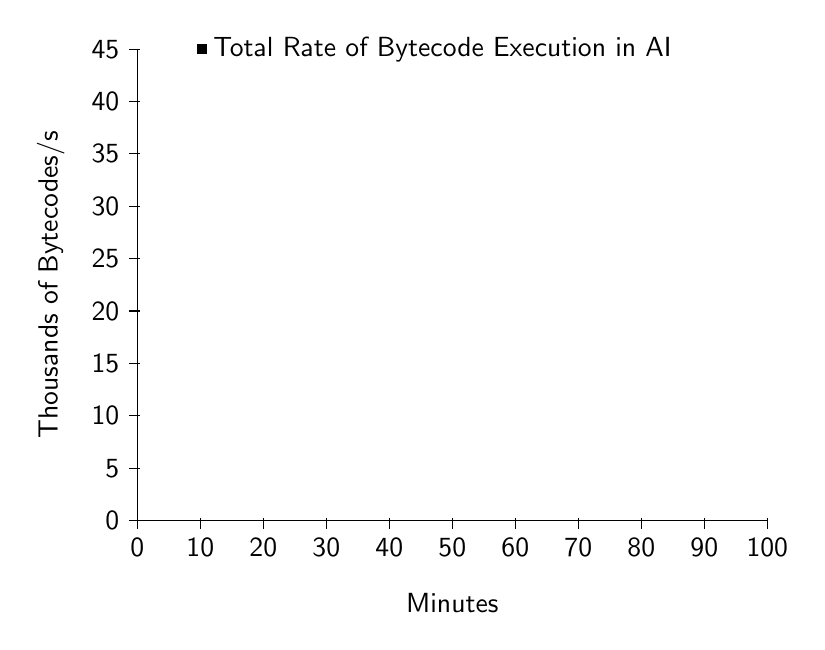
\begin{tikzpicture}[y=.133cm, x=\experimentxscale,font=\sffamily]
 	%axis
	\draw (0,0) -- coordinate (x axis mid) (\experimentxaxismax,0);
    	\draw (0,0) -- coordinate (y axis mid) (0,45);
    	%ticks
    	\foreach \x in {0,\experimentxaxispertick,...,\experimentxaxismax}
     		\draw (\x,1pt) -- (\x,-3pt)
			node[anchor=north] {\x};
    	\foreach \y in {0,5,...,45}
     		\draw (1pt,\y) -- (-3pt,\y) 
     			node[anchor=east] {\y}; 
	%labels      
	\node[below=0.8cm] at (x axis mid) {Minutes};
	\node[rotate=90, above=0.8cm] at (y axis mid) {Thousands of Bytecodes/s};

	%plots
	\draw plot[mark=square*, mark options={fill=black,scale=\experimentmarkscale}]
		file {data/mind_plot-Gripper-1-bytecode_count.data};
    
	%legend
	\begin{scope}[shift={(10,45)}]
	\draw (0,0) -- 
		plot[mark=square*, mark options={fill=black,scale=\experimentmarkscale}] (0.25,0) -- (0.5,0) 
		node[right]{Total Rate of Bytecode Execution in AI};
	\end{scope}
\end{tikzpicture}

\vspace{5mm}

\begin{tikzpicture}[y=1cm, x=\experimentxscale,font=\sffamily]
 	%axis
	\draw (0,0) -- coordinate (x axis mid) (\experimentxaxismax,0);
    	\draw (0,0) -- coordinate (y axis mid) (0,6);
    	%ticks
    	\foreach \x in {0,\experimentxaxispertick,...,\experimentxaxismax}
     		\draw (\x,1pt) -- (\x,-3pt)
			node[anchor=north] {\x};
    	\foreach \y in {0,1,...,6}
     		\draw (1pt,\y) -- (-3pt,\y)
     			node[anchor=east] {\y};
	%labels
	\node[below=0.8cm] at (x axis mid) {Minutes};
	\node[rotate=90, above=0.8cm] at (y axis mid) {Millions of Bytes/s};

	%plots
	\draw plot[mark=square*, mark options={fill=white,scale=\experimentmarkscale}]
		file {data/mind_plot-Gripper-1-bytes_allocated_count.data};
        
	%legend
	\begin{scope}[shift={(10,6)}]
	\draw (0,0) -- 
		plot[mark=square*, mark options={fill=white,scale=\experimentmarkscale}] (0.25,0) -- (0.5,0)
		node[right]{Total Rate of Memory Allocation in AI};
	\end{scope}
\end{tikzpicture}
\caption[Total rate of bytecode execution and memory allocation in the
  AI.]{Total rate of bytecode execution and memory allocation in the
  AI during a demonstration of mind initialization, plan execution,
  failure, physical learning, and reflective learning..}
\label{figure:mind_plot_data}
\end{figure}


% bytecode execution rate for each layer
\begin{figure}
\raggedleft
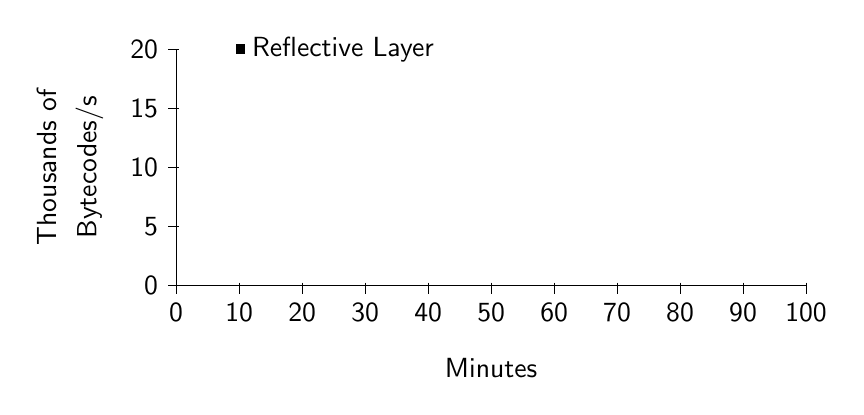
\begin{tikzpicture}[y=0.15cm, x=\experimentxscale,font=\sffamily]
 	%axis
	\draw (0,0) -- coordinate (x axis mid) (\experimentxaxismax,0);
    	\draw (0,0) -- coordinate (y axis mid) (0,20);
    	%ticks
    	\foreach \x in {0,\experimentxaxispertick,...,\experimentxaxismax}
     		\draw (\x,1pt) -- (\x,-3pt)
			node[anchor=north] {\x};
    	\foreach \y in {0,5,...,20}
     		\draw (1pt,\y) -- (-3pt,\y) 
     			node[anchor=east] {\y}; 
	%labels
	\node[below=0.8cm] at (x axis mid) {Minutes};
	\node[rotate=90, above=1.4cm] at (y axis mid) {Thousands of};
	\node[rotate=90, above=0.8cm] at (y axis mid) {Bytecodes/s};

	%plots
	\draw plot[mark=square*, mark options={scale=\experimentmarkscale}]
		file {data/mind_plot-Gripper-1-reflective-bytecode_count.data};
        
	%legend
	\begin{scope}[shift={(10,20)}] 
	\draw (0,0) -- 
		plot[mark=square*, mark options={fill=black,scale=\experimentmarkscale}] (0.25,0) -- (0.5,0)
		node[right]{Reflective Layer};
	\end{scope}
\end{tikzpicture}

\vspace{5mm}

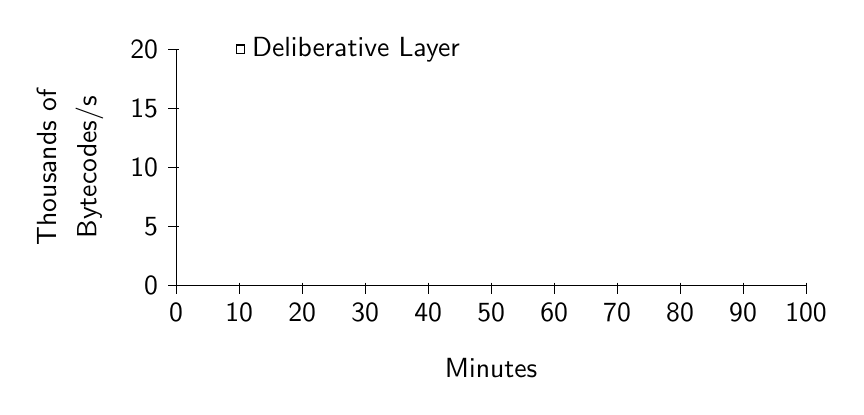
\begin{tikzpicture}[y=0.15cm, x=\experimentxscale,font=\sffamily]
 	%axis
	\draw (0,0) -- coordinate (x axis mid) (\experimentxaxismax,0);
    	\draw (0,0) -- coordinate (y axis mid) (0,20);
    	%ticks
    	\foreach \x in {0,\experimentxaxispertick,...,\experimentxaxismax}
     		\draw (\x,1pt) -- (\x,-3pt)
			node[anchor=north] {\x};
    	\foreach \y in {0,5,...,20}
     		\draw (1pt,\y) -- (-3pt,\y) 
     			node[anchor=east] {\y}; 
	%labels
	\node[below=0.8cm] at (x axis mid) {Minutes};
	\node[rotate=90, above=1.4cm] at (y axis mid) {Thousands of};
	\node[rotate=90, above=0.8cm] at (y axis mid) {Bytecodes/s};

	%plots
	\draw plot[mark=square*, mark options={fill=white,scale=\experimentmarkscale}]
		file {data/mind_plot-Gripper-1-deliberative-bytecode_count.data};
        
	%legend
	\begin{scope}[shift={(10,20)}] 
	\draw (0,0) -- 
		plot[mark=square*, mark options={fill=white,scale=\experimentmarkscale}] (0.25,0) -- (0.5,0)
		node[right]{Deliberative Layer};
	\end{scope}
\end{tikzpicture}

\vspace{5mm}

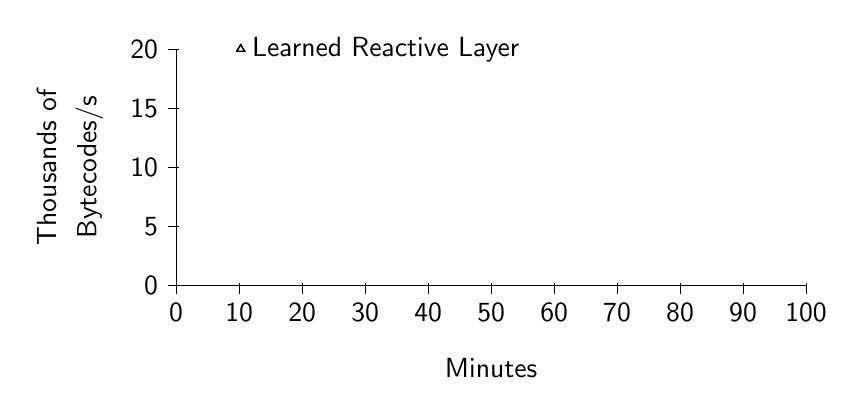
\begin{tikzpicture}[y=0.15cm, x=\experimentxscale,font=\sffamily]
 	%axis
	\draw (0,0) -- coordinate (x axis mid) (\experimentxaxismax,0);
    	\draw (0,0) -- coordinate (y axis mid) (0,20);
    	%ticks
    	\foreach \x in {0,\experimentxaxispertick,...,\experimentxaxismax}
     		\draw (\x,1pt) -- (\x,-3pt)
			node[anchor=north] {\x};
    	\foreach \y in {0,5,...,20}
     		\draw (1pt,\y) -- (-3pt,\y) 
     			node[anchor=east] {\y}; 
	%labels
	\node[below=0.8cm] at (x axis mid) {Minutes};
	\node[rotate=90, above=1.4cm] at (y axis mid) {Thousands of};
	\node[rotate=90, above=0.8cm] at (y axis mid) {Bytecodes/s};

	%plots
	\draw plot[mark=triangle*, mark options={fill=white,scale=\experimentmarkscale}]
		file {data/mind_plot-Gripper-1-learned_reactive-bytecode_count.data};
        
	%legend
	\begin{scope}[shift={(10,20)}] 
	\draw (0,0) -- 
		plot[mark=triangle*, mark options={fill=white,scale=\experimentmarkscale}] (0.25,0) -- (0.5,0)
		node[right]{Learned Reactive Layer};
	\end{scope}
\end{tikzpicture}

\vspace{5mm}

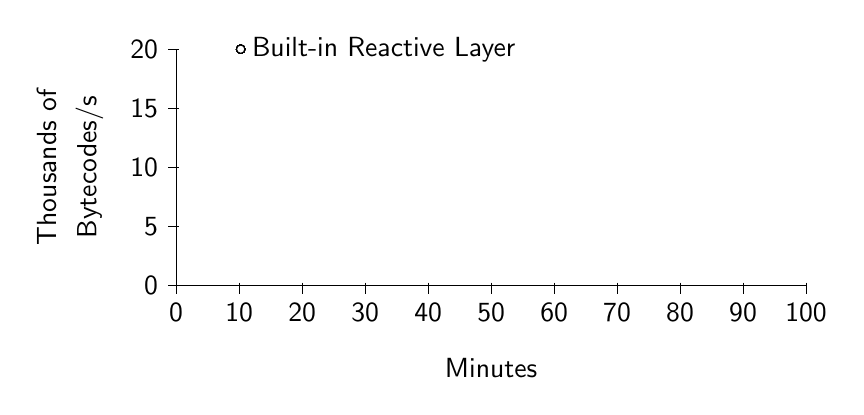
\begin{tikzpicture}[y=0.15cm, x=\experimentxscale,font=\sffamily]
 	%axis
	\draw (0,0) -- coordinate (x axis mid) (\experimentxaxismax,0);
    	\draw (0,0) -- coordinate (y axis mid) (0,20);
    	%ticks
    	\foreach \x in {0,\experimentxaxispertick,...,\experimentxaxismax}
     		\draw (\x,1pt) -- (\x,-3pt)
			node[anchor=north] {\x};
    	\foreach \y in {0,5,...,20}
     		\draw (1pt,\y) -- (-3pt,\y) 
     			node[anchor=east] {\y}; 
	%labels
	\node[below=0.8cm] at (x axis mid) {Minutes};
	\node[rotate=90, above=1.4cm] at (y axis mid) {Thousands of};
	\node[rotate=90, above=0.8cm] at (y axis mid) {Bytecodes/s};

	%plots
	\draw plot[mark=*, mark options={fill=white,scale=\experimentmarkscale}]
		file {data/mind_plot-Gripper-1-builtin_reactive-bytecode_count.data};
        
	%legend
	\begin{scope}[shift={(10,20)}] 
	\draw (0,0) -- 
		plot[mark=*, mark options={fill=white,scale=\experimentmarkscale}] (0.25,0) -- (0.5,0) 
		node[right]{Built-in Reactive Layer};
	\end{scope}
\end{tikzpicture}
\caption[Rate of bytecode execution in each layer of the AI during a
  demonstration.]{Rate of bytecode execution in each layer of the AI
  during a demonstration of mind initialization, plan execution,
  failure, physical learning, and reflective learning.}
\label{figure:mind_plot_data}
\end{figure}


% memory allocation rate for each layer
\begin{figure}
\raggedleft
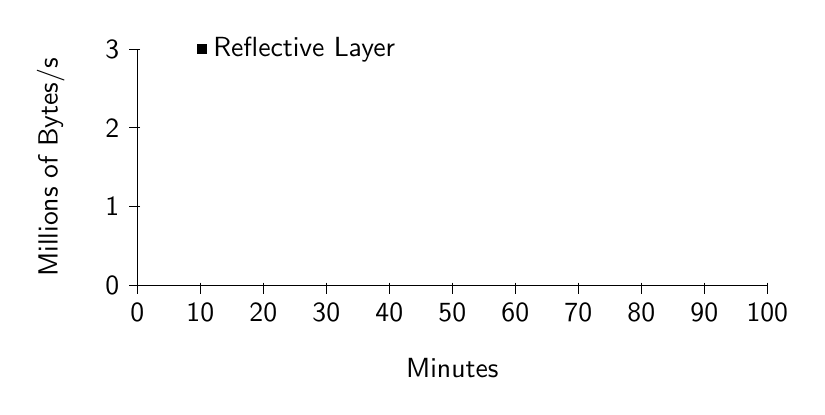
\begin{tikzpicture}[y=1cm, x=\experimentxscale,font=\sffamily]
 	%axis
	\draw (0,0) -- coordinate (x axis mid) (\experimentxaxismax,0);
    	\draw (0,0) -- coordinate (y axis mid) (0,3);
    	%ticks
    	\foreach \x in {0,\experimentxaxispertick,...,\experimentxaxismax}
     		\draw (\x,1pt) -- (\x,-3pt)
			node[anchor=north] {\x};
    	\foreach \y in {0,1,...,3}
     		\draw (1pt,\y) -- (-3pt,\y) 
     			node[anchor=east] {\y}; 
	%labels
	\node[below=0.8cm] at (x axis mid) {Minutes};
	\node[rotate=90, above=0.8cm] at (y axis mid) {Millions of Bytes/s};

	%plots
	\draw plot[mark=square*, mark options={scale=\experimentmarkscale}]
		file {data/mind_plot-Gripper-1-reflective-bytes_allocated_count.data};
        
	%legend
	\begin{scope}[shift={(10,3)}] 
	\draw (0,0) -- 
		plot[mark=square*, mark options={fill=black,scale=\experimentmarkscale}] (0.25,0) -- (0.5,0)
		node[right]{Reflective Layer};
	\end{scope}
\end{tikzpicture}

\vspace{5mm}

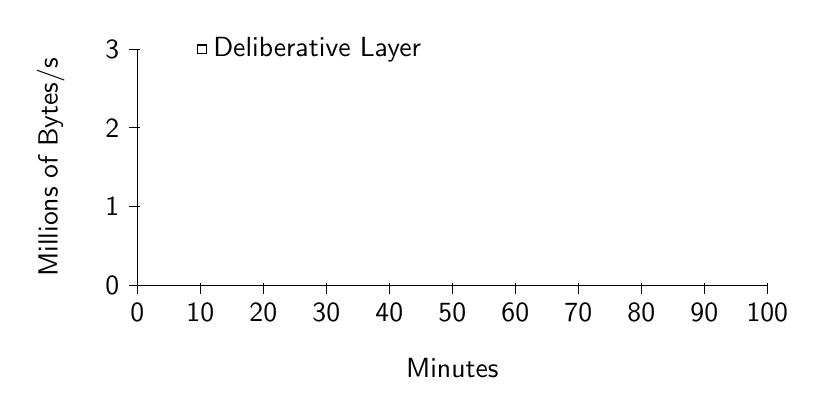
\begin{tikzpicture}[y=1cm, x=\experimentxscale,font=\sffamily]
 	%axis
	\draw (0,0) -- coordinate (x axis mid) (\experimentxaxismax,0);
    	\draw (0,0) -- coordinate (y axis mid) (0,3);
    	%ticks
    	\foreach \x in {0,\experimentxaxispertick,...,\experimentxaxismax}
     		\draw (\x,1pt) -- (\x,-3pt)
			node[anchor=north] {\x};
    	\foreach \y in {0,1,...,3}
     		\draw (1pt,\y) -- (-3pt,\y) 
     			node[anchor=east] {\y}; 
	%labels
	\node[below=0.8cm] at (x axis mid) {Minutes};
	\node[rotate=90, above=0.8cm] at (y axis mid) {Millions of Bytes/s};

	%plots
	\draw plot[mark=square*, mark options={fill=white,scale=\experimentmarkscale}]
		file {data/mind_plot-Gripper-1-deliberative-bytes_allocated_count.data};
        
	%legend
	\begin{scope}[shift={(10,3)}] 
	\draw (0,0) -- 
		plot[mark=square*, mark options={fill=white,scale=\experimentmarkscale}] (0.25,0) -- (0.5,0)
		node[right]{Deliberative Layer};
	\end{scope}
\end{tikzpicture}

\vspace{5mm}

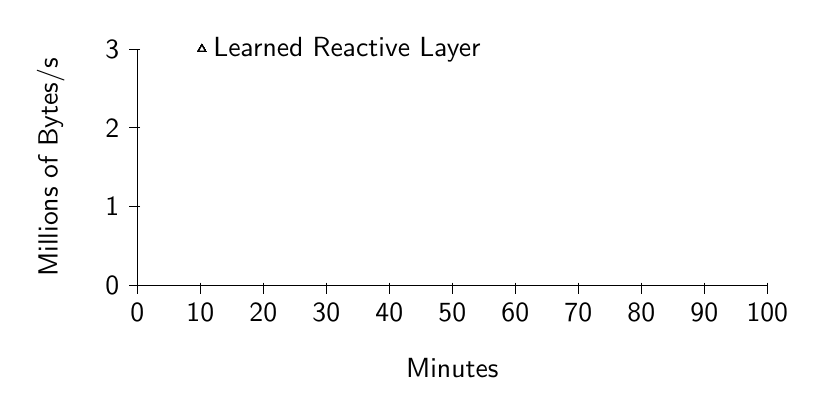
\begin{tikzpicture}[y=1cm, x=\experimentxscale,font=\sffamily]
 	%axis
	\draw (0,0) -- coordinate (x axis mid) (\experimentxaxismax,0);
    	\draw (0,0) -- coordinate (y axis mid) (0,3);
    	%ticks
    	\foreach \x in {0,\experimentxaxispertick,...,\experimentxaxismax}
     		\draw (\x,1pt) -- (\x,-3pt)
			node[anchor=north] {\x};
    	\foreach \y in {0,1,...,3}
     		\draw (1pt,\y) -- (-3pt,\y) 
     			node[anchor=east] {\y}; 
	%labels
	\node[below=0.8cm] at (x axis mid) {Minutes};
	\node[rotate=90, above=0.8cm] at (y axis mid) {Millions of Bytes/s};

	%plots
	\draw plot[mark=triangle*, mark options={fill=white,scale=\experimentmarkscale}]
		file {data/mind_plot-Gripper-1-learned_reactive-bytes_allocated_count.data};
        
	%legend
	\begin{scope}[shift={(10,3)}] 
	\draw (0,0) -- 
		plot[mark=triangle*, mark options={fill=white,scale=\experimentmarkscale}] (0.25,0) -- (0.5,0)
		node[right]{Learned Reactive Layer};
	\end{scope}
\end{tikzpicture}

\vspace{5mm}

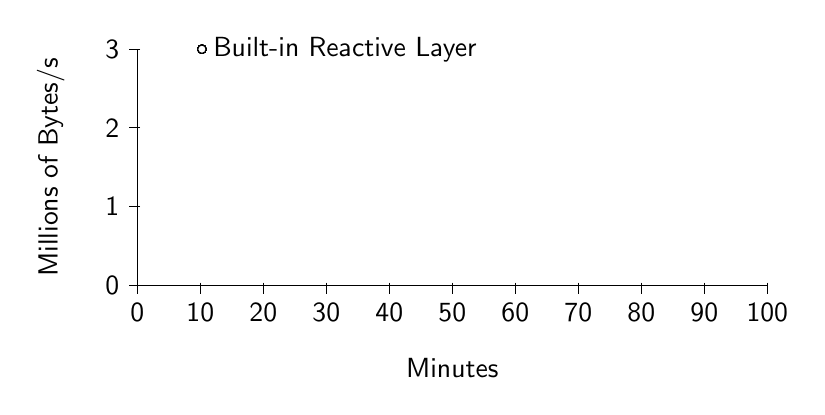
\begin{tikzpicture}[y=1cm, x=\experimentxscale,font=\sffamily]
 	%axis
	\draw (0,0) -- coordinate (x axis mid) (\experimentxaxismax,0);
    	\draw (0,0) -- coordinate (y axis mid) (0,3);
    	%ticks
    	\foreach \x in {0,\experimentxaxispertick,...,\experimentxaxismax}
     		\draw (\x,1pt) -- (\x,-3pt)
			node[anchor=north] {\x};
    	\foreach \y in {0,1,...,3}
     		\draw (1pt,\y) -- (-3pt,\y) 
     			node[anchor=east] {\y}; 
	%labels
	\node[below=0.8cm] at (x axis mid) {Minutes};
	\node[rotate=90, above=0.8cm] at (y axis mid) {Millions of Bytes/s};

	%plots
	\draw plot[mark=*, mark options={fill=white,scale=\experimentmarkscale}]
		file {data/mind_plot-Gripper-1-builtin_reactive-bytes_allocated_count.data};
        
	%legend
	\begin{scope}[shift={(10,3)}]
	\draw (0,0) -- 
		plot[mark=*, mark options={fill=white,scale=\experimentmarkscale}] (0.25,0) -- (0.5,0) 
		node[right]{Built-in Reactive Layer};
	\end{scope}
\end{tikzpicture}
\caption[Rate of memory allocation in each layer of the AI during a
  demonstration.]{Rate of memory allocation in each layer of the AI
  during a demonstration of mind initialization, plan execution,
  failure, physical learning, and reflective learning.}
\label{figure:mind_plot_data}
\end{figure}


% built-in reactive agency bytecode rate plots
\begin{figure}
\raggedleft
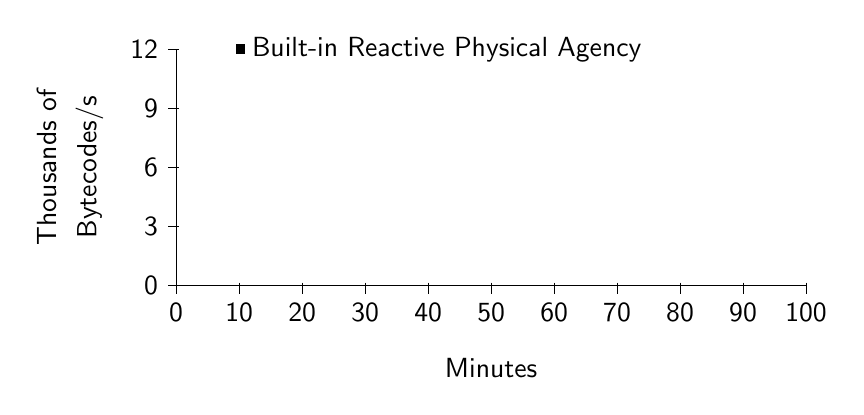
\begin{tikzpicture}[y=0.25cm, x=\experimentxscale,font=\sffamily]
 	%axis
	\draw (0,0) -- coordinate (x axis mid) (\experimentxaxismax,0);
    	\draw (0,0) -- coordinate (y axis mid) (0,12);
    	%ticks
    	\foreach \x in {0,\experimentxaxispertick,...,\experimentxaxismax}
     		\draw (\x,1pt) -- (\x,-3pt)
			node[anchor=north] {\x};
    	\foreach \y in {0,3,...,12}
     		\draw (1pt,\y) -- (-3pt,\y) 
     			node[anchor=east] {\y}; 
        
	%labels
	\node[below=0.8cm] at (x axis mid) {Minutes};
	\node[rotate=90, above=1.4cm] at (y axis mid) {Thousands of};
	\node[rotate=90, above=0.8cm] at (y axis mid) {Bytecodes/s};

	%plots
	\draw plot[mark=square*, mark options={fill=black,scale=\experimentmarkscale}]
		file {data/mind_plot-Gripper-1-builtin_reactive-physical-bytecode_count.data};
        
	%legend
	\begin{scope}[shift={(10,12)}]
	\draw (0,0) -- 
		plot[mark=square*, mark options={fill=black,scale=\experimentmarkscale}] (0.25,0) -- (0.5,0) 
		node[right]{Built-in Reactive Physical Agency};
	\end{scope}
\end{tikzpicture}

\vspace{5mm}

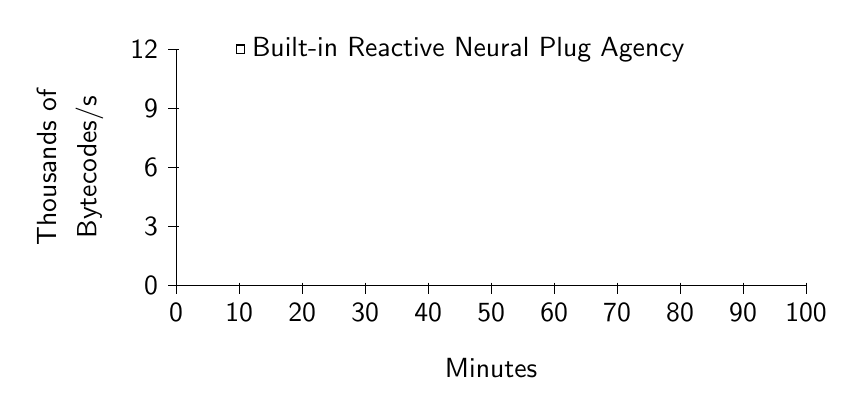
\begin{tikzpicture}[y=0.25cm, x=\experimentxscale,font=\sffamily]
 	%axis
	\draw (0,0) -- coordinate (x axis mid) (\experimentxaxismax,0);
    	\draw (0,0) -- coordinate (y axis mid) (0,12);
    	%ticks
    	\foreach \x in {0,\experimentxaxispertick,...,\experimentxaxismax}
     		\draw (\x,1pt) -- (\x,-3pt)
			node[anchor=north] {\x};
    	\foreach \y in {0,3,...,12}
     		\draw (1pt,\y) -- (-3pt,\y) 
     			node[anchor=east] {\y}; 
        
	%labels
	\node[below=0.8cm] at (x axis mid) {Minutes};
	\node[rotate=90, above=1.4cm] at (y axis mid) {Thousands of};
	\node[rotate=90, above=0.8cm] at (y axis mid) {Bytecodes/s};

	%plots
	\draw plot[mark=square*, mark options={fill=white,scale=\experimentmarkscale}]
		file {data/mind_plot-Gripper-1-builtin_reactive-neural_plug-bytecode_count.data};
        
	%legend
	\begin{scope}[shift={(10,12)}]
	\draw (0,0) -- 
		plot[mark=square*, mark options={fill=white,scale=\experimentmarkscale}] (0.25,0) -- (0.5,0) 
		node[right]{Built-in Reactive Neural Plug Agency};
	\end{scope}
\end{tikzpicture}

\vspace{5mm}

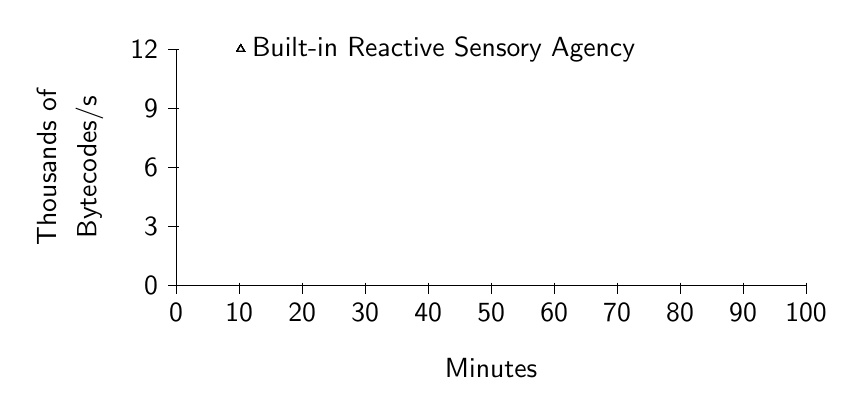
\begin{tikzpicture}[y=0.25cm, x=\experimentxscale,font=\sffamily]
 	%axis
	\draw (0,0) -- coordinate (x axis mid) (\experimentxaxismax,0);
    	\draw (0,0) -- coordinate (y axis mid) (0,12);
    	%ticks
    	\foreach \x in {0,\experimentxaxispertick,...,\experimentxaxismax}
     		\draw (\x,1pt) -- (\x,-3pt)
			node[anchor=north] {\x};
    	\foreach \y in {0,3,...,12}
     		\draw (1pt,\y) -- (-3pt,\y) 
     			node[anchor=east] {\y}; 
        
	%labels
	\node[below=0.8cm] at (x axis mid) {Minutes};
	\node[rotate=90, above=1.4cm] at (y axis mid) {Thousands of};
	\node[rotate=90, above=0.8cm] at (y axis mid) {Bytecodes/s};

	%plots
	\draw plot[mark=triangle*, mark options={fill=white,scale=\experimentmarkscale}]
		file {data/mind_plot-Gripper-1-builtin_reactive-sensory-bytecode_count.data};
        
	%legend
	\begin{scope}[shift={(10,12)}]
	\draw (0,0) -- 
		plot[mark=triangle*, mark options={fill=white,scale=\experimentmarkscale}] (0.25,0) -- (0.5,0) 
		node[right]{Built-in Reactive Sensory Agency};
	\end{scope}
\end{tikzpicture}
\caption[Rate of bytecode execution in each agency of the built-in
  reactive layer of the AI during a demonstration.]{Rate of bytecode
  execution in each agency of the built-in reactive layer of the AI
  during a demonstration of mind initialization, plan execution,
  failure, physical learning, and reflective learning.}
\label{figure:mind_plot_data}
\end{figure}


% built-in reactive agency memory allocation rate plots
\begin{figure}
\raggedleft
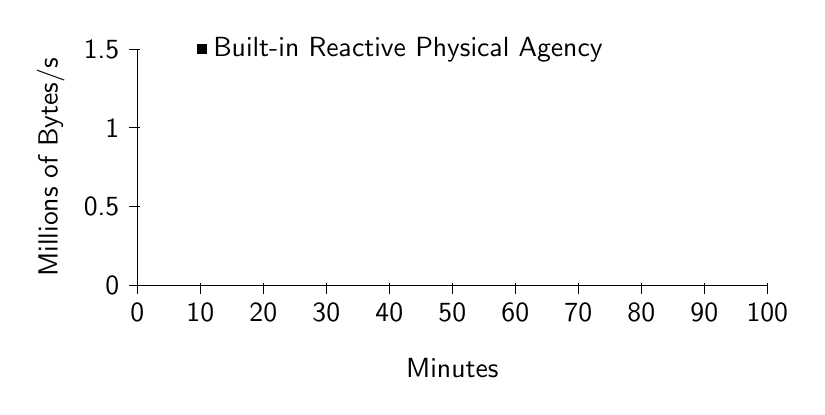
\begin{tikzpicture}[y=2cm, x=\experimentxscale,font=\sffamily]
 	%axis
	\draw (0,0) -- coordinate (x axis mid) (\experimentxaxismax,0);
    	\draw (0,0) -- coordinate (y axis mid) (0,1.5);
    	%ticks
    	\foreach \x in {0,\experimentxaxispertick,...,\experimentxaxismax}
     		\draw (\x,1pt) -- (\x,-3pt)
			node[anchor=north] {\x};
    	\foreach \y in {0,0.5,...,1.5}
     		\draw (1pt,\y) -- (-3pt,\y) 
     			node[anchor=east] {\y}; 
        
	%labels
	\node[below=0.8cm] at (x axis mid) {Minutes};
	\node[rotate=90, above=0.8cm] at (y axis mid) {Millions of Bytes/s};

	%plots
	\draw plot[mark=square*, mark options={fill=black,scale=\experimentmarkscale}]
		file {data/mind_plot-Gripper-1-builtin_reactive-physical-bytes_allocated_count.data};
        
	%legend
	\begin{scope}[shift={(10,1.5)}]
	\draw (0,0) -- 
		plot[mark=square*, mark options={fill=black,scale=\experimentmarkscale}] (0.25,0) -- (0.5,0) 
		node[right]{Built-in Reactive Physical Agency};
	\end{scope}
\end{tikzpicture}

\vspace{5mm}

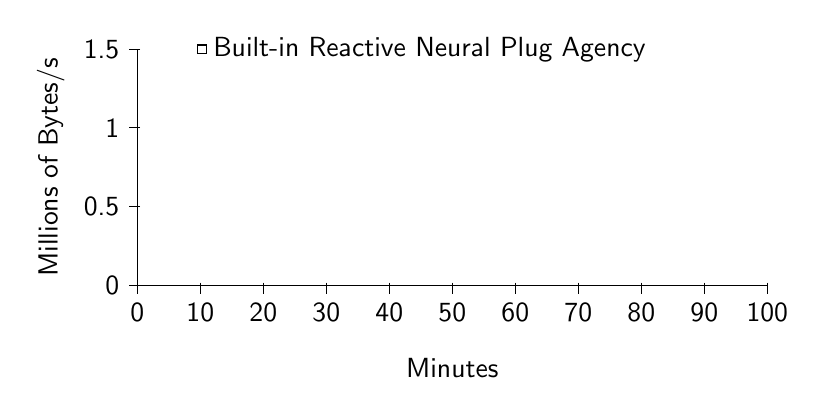
\begin{tikzpicture}[y=2cm, x=\experimentxscale,font=\sffamily]
 	%axis
	\draw (0,0) -- coordinate (x axis mid) (\experimentxaxismax,0);
    	\draw (0,0) -- coordinate (y axis mid) (0,1.5);
    	%ticks
    	\foreach \x in {0,\experimentxaxispertick,...,\experimentxaxismax}
     		\draw (\x,1pt) -- (\x,-3pt)
			node[anchor=north] {\x};
    	\foreach \y in {0,0.5,...,1.5}
     		\draw (1pt,\y) -- (-3pt,\y) 
     			node[anchor=east] {\y}; 
        
	%labels
	\node[below=0.8cm] at (x axis mid) {Minutes};
	\node[rotate=90, above=0.8cm] at (y axis mid) {Millions of Bytes/s};
        
	%plots
	\draw plot[mark=square*, mark options={fill=white,scale=\experimentmarkscale}]
		file {data/mind_plot-Gripper-1-builtin_reactive-neural_plug-bytes_allocated_count.data};
        
	%legend
	\begin{scope}[shift={(10,1.5)}]
	\draw (0,0) -- 
		plot[mark=square*, mark options={fill=white,scale=\experimentmarkscale}] (0.25,0) -- (0.5,0) 
		node[right]{Built-in Reactive Neural Plug Agency};
	\end{scope}
\end{tikzpicture}

\vspace{5mm}

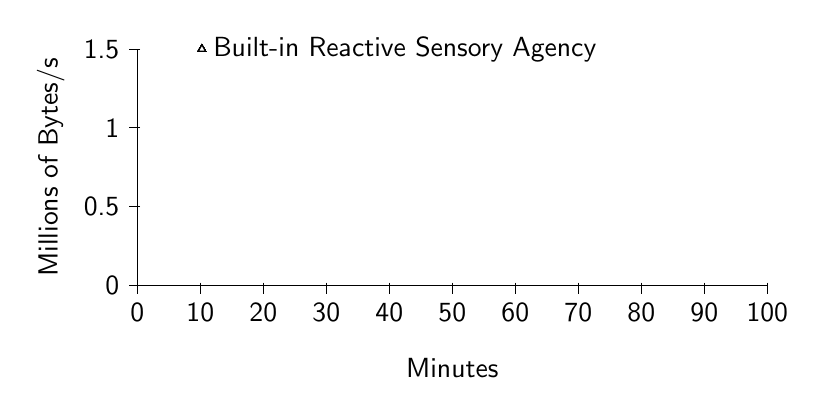
\begin{tikzpicture}[y=2cm, x=\experimentxscale,font=\sffamily]
 	%axis
	\draw (0,0) -- coordinate (x axis mid) (\experimentxaxismax,0);
    	\draw (0,0) -- coordinate (y axis mid) (0,1.5);
    	%ticks
    	\foreach \x in {0,\experimentxaxispertick,...,\experimentxaxismax}
     		\draw (\x,1pt) -- (\x,-3pt)
			node[anchor=north] {\x};
    	\foreach \y in {0,0.5,...,1.5}
     		\draw (1pt,\y) -- (-3pt,\y) 
     			node[anchor=east] {\y}; 
        
	%labels
	\node[below=0.8cm] at (x axis mid) {Minutes};
	\node[rotate=90, above=0.8cm] at (y axis mid) {Millions of Bytes/s};

	%plots
	\draw plot[mark=triangle*, mark options={fill=white,scale=\experimentmarkscale}]
		file {data/mind_plot-Gripper-1-builtin_reactive-sensory-bytes_allocated_count.data};
        
	%legend
	\begin{scope}[shift={(10,1.5)}]
	\draw (0,0) -- 
		plot[mark=triangle*, mark options={fill=white,scale=\experimentmarkscale}] (0.25,0) -- (0.5,0) 
		node[right]{Built-in Reactive Sensory Agency};
	\end{scope}
\end{tikzpicture}
\caption[Rate of memory allocation in each agency of the built-in
  reactive layer of the AI during a demonstration.]{Rate of memory
  allocation in each agency of the built-in reactive layer of the AI
  during a demonstration of mind initialization, plan execution,
  failure, physical learning, and reflective learning.}
\label{figure:mind_plot_data}
\end{figure}


% learned reactive agency bytecode rate plots
\begin{figure}
\raggedleft
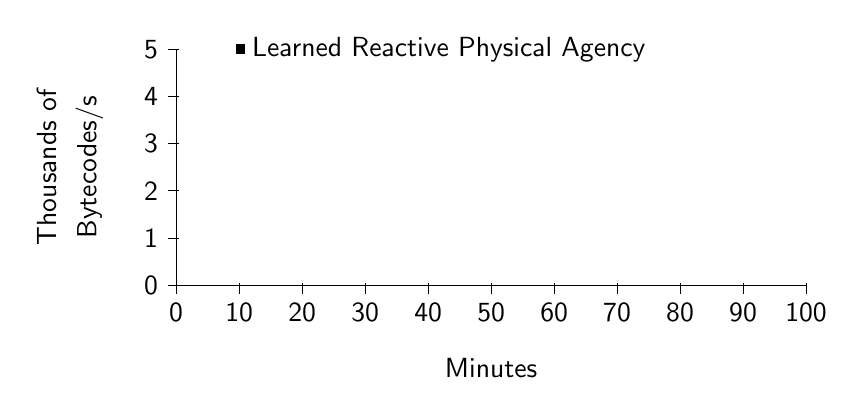
\begin{tikzpicture}[y=0.6cm, x=\experimentxscale,font=\sffamily]
 	%axis
	\draw (0,0) -- coordinate (x axis mid) (\experimentxaxismax,0);
    	\draw (0,0) -- coordinate (y axis mid) (0,5);
    	%ticks
    	\foreach \x in {0,\experimentxaxispertick,...,\experimentxaxismax}
     		\draw (\x,1pt) -- (\x,-3pt)
			node[anchor=north] {\x};
    	\foreach \y in {0,1,...,5}
     		\draw (1pt,\y) -- (-3pt,\y) 
     			node[anchor=east] {\y}; 
        
	%labels
	\node[below=0.8cm] at (x axis mid) {Minutes};
	\node[rotate=90, above=1.4cm] at (y axis mid) {Thousands of};
	\node[rotate=90, above=0.8cm] at (y axis mid) {Bytecodes/s};

	%plots
	\draw plot[mark=square*, mark options={fill=black,scale=\experimentmarkscale}]
		file {data/mind_plot-Gripper-1-learned_reactive-physical-bytecode_count.data};
        
	%legend
	\begin{scope}[shift={(10,5)}]
	\draw (0,0) -- 
		plot[mark=square*, mark options={fill=black,scale=\experimentmarkscale}] (0.25,0) -- (0.5,0) 
		node[right]{Learned Reactive Physical Agency};
	\end{scope}
\end{tikzpicture}

\vspace{5mm}

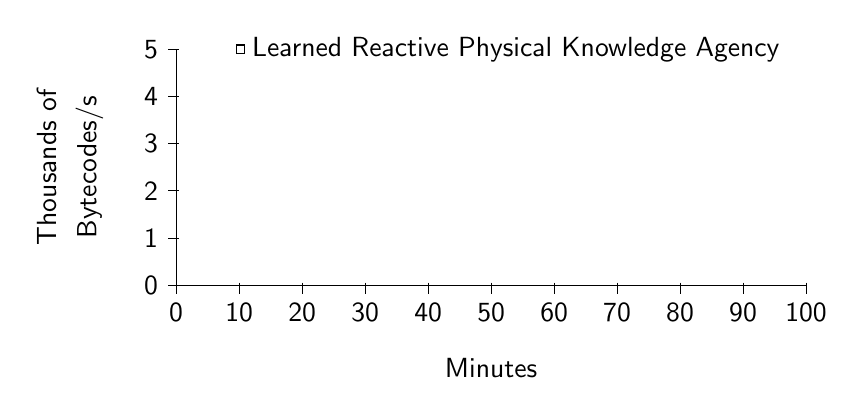
\begin{tikzpicture}[y=0.6cm, x=\experimentxscale,font=\sffamily]
 	%axis
	\draw (0,0) -- coordinate (x axis mid) (\experimentxaxismax,0);
    	\draw (0,0) -- coordinate (y axis mid) (0,5);
    	%ticks
    	\foreach \x in {0,\experimentxaxispertick,...,\experimentxaxismax}
     		\draw (\x,1pt) -- (\x,-3pt)
			node[anchor=north] {\x};
    	\foreach \y in {0,1,...,5}
     		\draw (1pt,\y) -- (-3pt,\y) 
     			node[anchor=east] {\y}; 
        
	%labels
	\node[below=0.8cm] at (x axis mid) {Minutes};
	\node[rotate=90, above=1.4cm] at (y axis mid) {Thousands of};
	\node[rotate=90, above=0.8cm] at (y axis mid) {Bytecodes/s};

	%plots
	\draw plot[mark=square*, mark options={fill=white,scale=\experimentmarkscale}]
		file {data/mind_plot-Gripper-1-learned_reactive-physical_knowledge-bytecode_count.data};
        
	%legend
	\begin{scope}[shift={(10,5)}]
	\draw (0,0) -- 
		plot[mark=square*, mark options={fill=white,scale=\experimentmarkscale}] (0.25,0) -- (0.5,0) 
		node[right]{Learned Reactive Physical Knowledge Agency};
	\end{scope}
\end{tikzpicture}

\vspace{5mm}

% learned reactive agency memory allocation rate plots
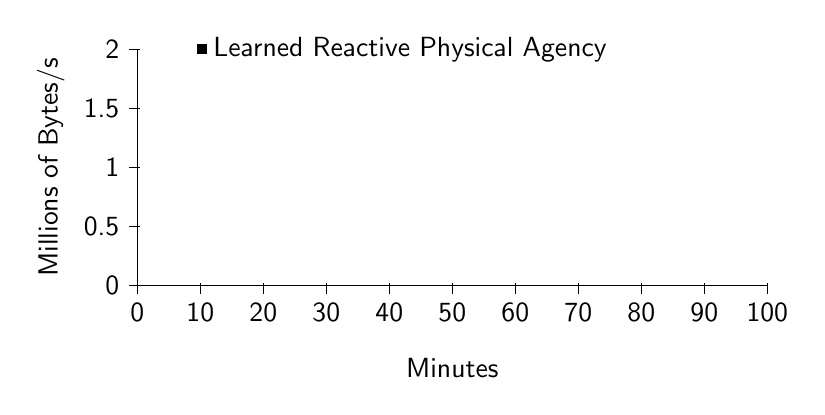
\begin{tikzpicture}[y=1.5cm, x=\experimentxscale,font=\sffamily]
 	%axis
	\draw (0,0) -- coordinate (x axis mid) (\experimentxaxismax,0);
    	\draw (0,0) -- coordinate (y axis mid) (0,2);
    	%ticks
    	\foreach \x in {0,\experimentxaxispertick,...,\experimentxaxismax}
     		\draw (\x,1pt) -- (\x,-3pt)
			node[anchor=north] {\x};
    	\foreach \y in {0,0.5,...,2}
     		\draw (1pt,\y) -- (-3pt,\y) 
     			node[anchor=east] {\y}; 
        
	%labels
	\node[below=0.8cm] at (x axis mid) {Minutes};
	\node[rotate=90, above=0.8cm] at (y axis mid) {Millions of Bytes/s};

	%plots
	\draw plot[mark=square*, mark options={fill=black,scale=\experimentmarkscale}]
		file {data/mind_plot-Gripper-1-learned_reactive-physical-bytes_allocated_count.data};
        
	%legend
	\begin{scope}[shift={(10,2)}]
	\draw (0,0) -- 
		plot[mark=square*, mark options={fill=black,scale=\experimentmarkscale}] (0.25,0) -- (0.5,0) 
		node[right]{Learned Reactive Physical Agency};
	\end{scope}
\end{tikzpicture}

\vspace{5mm}

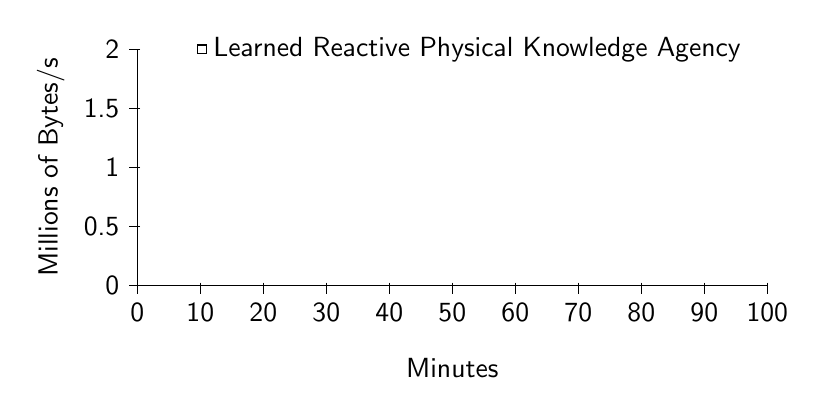
\begin{tikzpicture}[y=1.5cm, x=\experimentxscale,font=\sffamily]
 	%axis
	\draw (0,0) -- coordinate (x axis mid) (\experimentxaxismax,0);
    	\draw (0,0) -- coordinate (y axis mid) (0,2);
    	%ticks
    	\foreach \x in {0,\experimentxaxispertick,...,\experimentxaxismax}
     		\draw (\x,1pt) -- (\x,-3pt)
			node[anchor=north] {\x};
    	\foreach \y in {0,0.5,...,2}
     		\draw (1pt,\y) -- (-3pt,\y) 
     			node[anchor=east] {\y}; 
        
	%labels
	\node[below=0.8cm] at (x axis mid) {Minutes};
	\node[rotate=90, above=0.8cm] at (y axis mid) {Millions of Bytes/s};

	%plots
	\draw plot[mark=square*, mark options={fill=white,scale=\experimentmarkscale}]
		file {data/mind_plot-Gripper-1-learned_reactive-physical_knowledge-bytecode_count.data};
        
	%legend
	\begin{scope}[shift={(10,2)}]
	\draw (0,0) -- 
		plot[mark=square*, mark options={fill=white,scale=\experimentmarkscale}] (0.25,0) -- (0.5,0) 
		node[right]{Learned Reactive Physical Knowledge Agency};
	\end{scope}
\end{tikzpicture}

\caption[Rate of bytecode execution and memory allocation in each
  agency of the learned reactive layer of the AI during a
  demonstration.]{Rate of bytecode execution and memory allocation in
  each agency of the learned reactive layer of the AI during a
  demonstration of mind initialization, plan execution, failure,
  physical learning, and reflective learning.}
\label{figure:mind_plot_data}
\end{figure}



% deliberative agency bytecode rate plots
\begin{figure}
\raggedleft
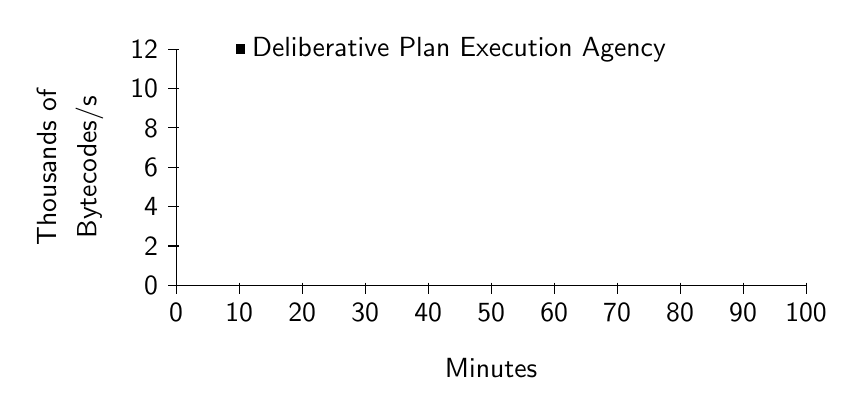
\begin{tikzpicture}[y=0.25cm, x=\experimentxscale,font=\sffamily]
 	%axis
	\draw (0,0) -- coordinate (x axis mid) (\experimentxaxismax,0);
    	\draw (0,0) -- coordinate (y axis mid) (0,12);
    	%ticks
    	\foreach \x in {0,\experimentxaxispertick,...,\experimentxaxismax}
     		\draw (\x,1pt) -- (\x,-3pt)
			node[anchor=north] {\x};
    	\foreach \y in {0,2,...,12}
     		\draw (1pt,\y) -- (-3pt,\y) 
     			node[anchor=east] {\y}; 
        
	%labels
	\node[below=0.8cm] at (x axis mid) {Minutes};
	\node[rotate=90, above=1.4cm] at (y axis mid) {Thousands of};
	\node[rotate=90, above=0.8cm] at (y axis mid) {Bytecodes/s};

	%plots
	\draw plot[mark=square*, mark options={fill=black,scale=\experimentmarkscale}]
		file {data/mind_plot-Gripper-1-deliberative-execution-bytecode_count.data};
        
	%legend
	\begin{scope}[shift={(10,12)}]
	\draw (0,0) -- 
		plot[mark=square*, mark options={fill=black,scale=\experimentmarkscale}] (0.25,0) -- (0.5,0) 
		node[right]{Deliberative Plan Execution Agency};
	\end{scope}
\end{tikzpicture}

\vspace{5mm}

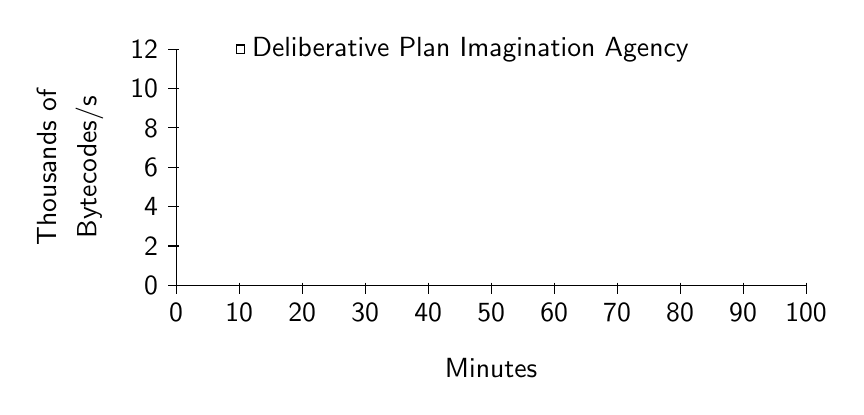
\begin{tikzpicture}[y=0.25cm, x=\experimentxscale,font=\sffamily]
 	%axis
	\draw (0,0) -- coordinate (x axis mid) (\experimentxaxismax,0);
    	\draw (0,0) -- coordinate (y axis mid) (0,12);
    	%ticks
    	\foreach \x in {0,\experimentxaxispertick,...,\experimentxaxismax}
     		\draw (\x,1pt) -- (\x,-3pt)
			node[anchor=north] {\x};
    	\foreach \y in {0,2,...,12}
     		\draw (1pt,\y) -- (-3pt,\y) 
     			node[anchor=east] {\y}; 
        
	%labels
	\node[below=0.8cm] at (x axis mid) {Minutes};
	\node[rotate=90, above=1.4cm] at (y axis mid) {Thousands of};
	\node[rotate=90, above=0.8cm] at (y axis mid) {Bytecodes/s};

	%plots
	\draw plot[mark=square*, mark options={fill=white,scale=\experimentmarkscale}]
		file {data/mind_plot-Gripper-1-deliberative-imagination-bytecode_count.data};
        
	%legend
	\begin{scope}[shift={(10,12)}]
	\draw (0,0) -- 
		plot[mark=square*, mark options={fill=white,scale=\experimentmarkscale}] (0.25,0) -- (0.5,0) 
		node[right]{Deliberative Plan Imagination Agency};
	\end{scope}
\end{tikzpicture}

\vspace{5mm}

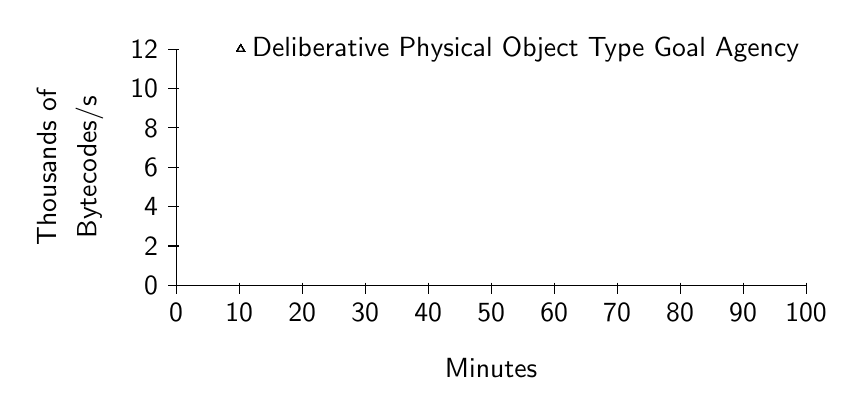
\begin{tikzpicture}[y=0.25cm, x=\experimentxscale,font=\sffamily]
 	%axis
	\draw (0,0) -- coordinate (x axis mid) (\experimentxaxismax,0);
    	\draw (0,0) -- coordinate (y axis mid) (0,12);
    	%ticks
    	\foreach \x in {0,\experimentxaxispertick,...,\experimentxaxismax}
     		\draw (\x,1pt) -- (\x,-3pt)
			node[anchor=north] {\x};
    	\foreach \y in {0,2,...,12}
     		\draw (1pt,\y) -- (-3pt,\y) 
     			node[anchor=east] {\y}; 
        
	%labels
	\node[below=0.8cm] at (x axis mid) {Minutes};
	\node[rotate=90, above=1.4cm] at (y axis mid) {Thousands of};
	\node[rotate=90, above=0.8cm] at (y axis mid) {Bytecodes/s};

	%plots
	\draw plot[mark=triangle*, mark options={fill=white,scale=\experimentmarkscale}]
		file {data/mind_plot-Gripper-1-deliberative-physical_object_type_goal-bytecode_count.data};
        
	%legend
	\begin{scope}[shift={(10,12)}]
	\draw (0,0) -- 
		plot[mark=triangle*, mark options={fill=white,scale=\experimentmarkscale}] (0.25,0) -- (0.5,0) 
		node[right]{Deliberative Physical Object Type Goal Agency};
	\end{scope}
\end{tikzpicture}

\vspace{5mm}

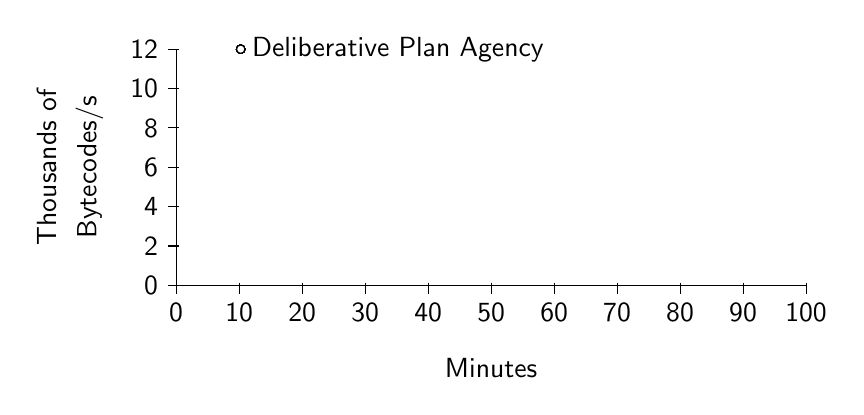
\begin{tikzpicture}[y=0.25cm, x=\experimentxscale,font=\sffamily]
 	%axis
	\draw (0,0) -- coordinate (x axis mid) (\experimentxaxismax,0);
    	\draw (0,0) -- coordinate (y axis mid) (0,12);
    	%ticks
    	\foreach \x in {0,\experimentxaxispertick,...,\experimentxaxismax}
     		\draw (\x,1pt) -- (\x,-3pt)
			node[anchor=north] {\x};
    	\foreach \y in {0,2,...,12}
     		\draw (1pt,\y) -- (-3pt,\y) 
     			node[anchor=east] {\y}; 
	%labels
	\node[below=0.8cm] at (x axis mid) {Minutes};
	\node[rotate=90, above=1.4cm] at (y axis mid) {Thousands of};
	\node[rotate=90, above=0.8cm] at (y axis mid) {Bytecodes/s};

	%plots
	\draw plot[mark=*, mark options={fill=white,scale=\experimentmarkscale}]
		file {data/mind_plot-Gripper-1-deliberative-plan-bytecode_count.data};
        
	%legend
	\begin{scope}[shift={(10,12)}]
	\draw (0,0) -- 
		plot[mark=*, mark options={fill=white,scale=\experimentmarkscale}] (0.25,0) -- (0.5,0) 
		node[right]{Deliberative Plan Agency};
	\end{scope}
\end{tikzpicture}
\caption[Rate of bytecode execution in each agency of the deliberative
  layer of the AI during a demonstration.]{Rate of bytecode execution
  in each agency of the deliberative layer of the AI during a
  demonstration of mind initialization, plan execution, failure,
  physical learning, and reflective learning.}
\label{figure:mind_plot_data}
\end{figure}


% deliberative agency memory allocation rate plots
\begin{figure}
\raggedleft
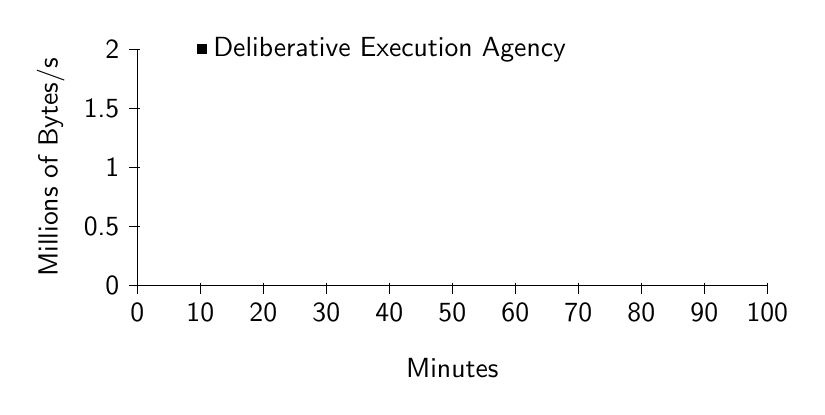
\begin{tikzpicture}[y=1.5cm, x=\experimentxscale,font=\sffamily]
 	%axis
	\draw (0,0) -- coordinate (x axis mid) (\experimentxaxismax,0);
    	\draw (0,0) -- coordinate (y axis mid) (0,2);
    	%ticks
    	\foreach \x in {0,\experimentxaxispertick,...,\experimentxaxismax}
     		\draw (\x,1pt) -- (\x,-3pt)
			node[anchor=north] {\x};
    	\foreach \y in {0,0.5,...,2}
     		\draw (1pt,\y) -- (-3pt,\y) 
     			node[anchor=east] {\y}; 
        
	%labels
	\node[below=0.8cm] at (x axis mid) {Minutes};
	\node[rotate=90, above=0.8cm] at (y axis mid) {Millions of Bytes/s};

	%plots
	\draw plot[mark=square*, mark options={fill=black,scale=\experimentmarkscale}]
		file {data/mind_plot-Gripper-1-deliberative-execution-bytes_allocated_count.data};
        
	%legend
	\begin{scope}[shift={(10,2)}]
	\draw (0,0) -- 
		plot[mark=square*, mark options={fill=black,scale=\experimentmarkscale}] (0.25,0) -- (0.5,0) 
		node[right]{Deliberative Execution Agency};
	\end{scope}
\end{tikzpicture}

\vspace{5mm}

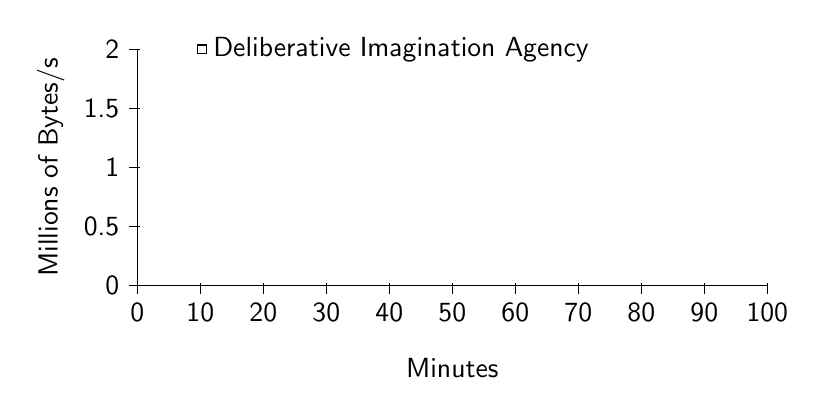
\begin{tikzpicture}[y=1.5cm, x=\experimentxscale,font=\sffamily]
 	%axis
	\draw (0,0) -- coordinate (x axis mid) (\experimentxaxismax,0);
    	\draw (0,0) -- coordinate (y axis mid) (0,2);
    	%ticks
    	\foreach \x in {0,\experimentxaxispertick,...,\experimentxaxismax}
     		\draw (\x,1pt) -- (\x,-3pt)
			node[anchor=north] {\x};
    	\foreach \y in {0,0.5,...,2}
     		\draw (1pt,\y) -- (-3pt,\y) 
     			node[anchor=east] {\y}; 
        
	%labels
	\node[below=0.8cm] at (x axis mid) {Minutes};
	\node[rotate=90, above=0.8cm] at (y axis mid) {Millions of Bytes/s};
        
	%plots
	\draw plot[mark=square*, mark options={fill=white,scale=\experimentmarkscale}]
		file {data/mind_plot-Gripper-1-deliberative-imagination-bytes_allocated_count.data};
        
	%legend
	\begin{scope}[shift={(10,2)}]
	\draw (0,0) -- 
		plot[mark=square*, mark options={fill=white,scale=\experimentmarkscale}] (0.25,0) -- (0.5,0) 
		node[right]{Deliberative Imagination Agency};
	\end{scope}
\end{tikzpicture}

\vspace{5mm}

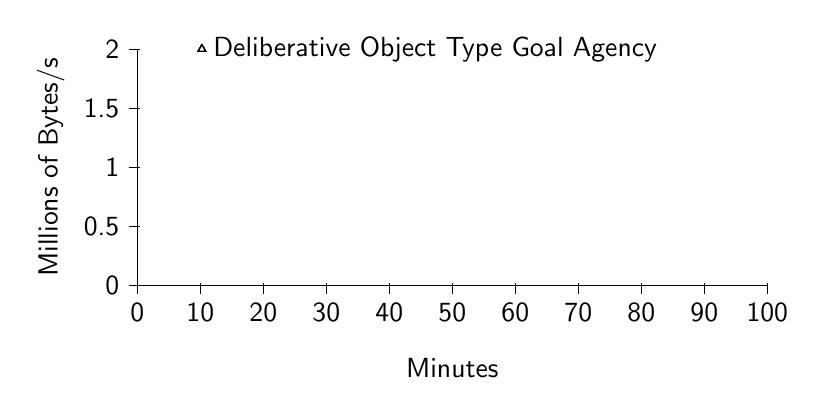
\begin{tikzpicture}[y=1.5cm, x=\experimentxscale,font=\sffamily]
 	%axis
	\draw (0,0) -- coordinate (x axis mid) (\experimentxaxismax,0);
    	\draw (0,0) -- coordinate (y axis mid) (0,2);
    	%ticks
    	\foreach \x in {0,\experimentxaxispertick,...,\experimentxaxismax}
     		\draw (\x,1pt) -- (\x,-3pt)
			node[anchor=north] {\x};
    	\foreach \y in {0,0.5,...,2}
     		\draw (1pt,\y) -- (-3pt,\y) 
     			node[anchor=east] {\y}; 
        
	%labels
	\node[below=0.8cm] at (x axis mid) {Minutes};
	\node[rotate=90, above=0.8cm] at (y axis mid) {Millions of Bytes/s};

	%plots
	\draw plot[mark=triangle*, mark options={fill=white,scale=\experimentmarkscale}]
		file {data/mind_plot-Gripper-1-deliberative-physical_object_type_goal-bytes_allocated_count.data};
        
	%legend
	\begin{scope}[shift={(10,2)}]
	\draw (0,0) -- 
		plot[mark=triangle*, mark options={fill=white,scale=\experimentmarkscale}] (0.25,0) -- (0.5,0) 
		node[right]{Deliberative Object Type Goal Agency};
	\end{scope}
\end{tikzpicture}

\vspace{5mm}

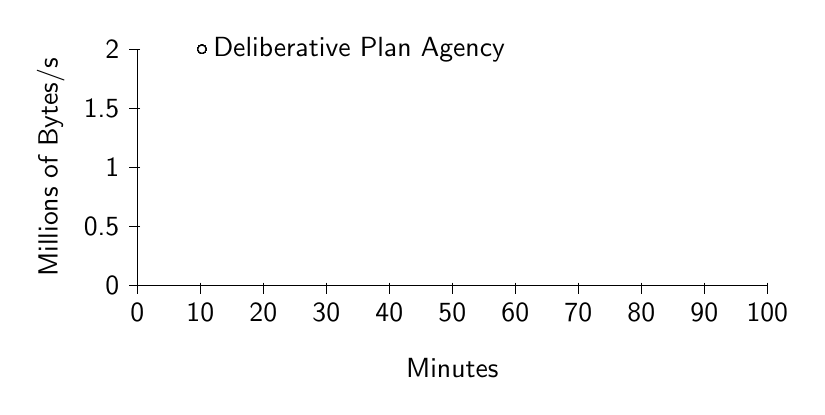
\begin{tikzpicture}[y=1.5cm, x=\experimentxscale,font=\sffamily]
 	%axis
	\draw (0,0) -- coordinate (x axis mid) (\experimentxaxismax,0);
    	\draw (0,0) -- coordinate (y axis mid) (0,2);
    	%ticks
    	\foreach \x in {0,\experimentxaxispertick,...,\experimentxaxismax}
     		\draw (\x,1pt) -- (\x,-3pt)
			node[anchor=north] {\x};
    	\foreach \y in {0,0.5,...,2}
     		\draw (1pt,\y) -- (-3pt,\y) 
     			node[anchor=east] {\y}; 
        
	%labels
	\node[below=0.8cm] at (x axis mid) {Minutes};
	\node[rotate=90, above=0.8cm] at (y axis mid) {Millions of Bytes/s};

	%plots
	\draw plot[mark=*, mark options={fill=white,scale=\experimentmarkscale}]
		file {data/mind_plot-Gripper-1-deliberative-plan-bytes_allocated_count.data};
        
	%legend
	\begin{scope}[shift={(10,2)}]
	\draw (0,0) -- 
		plot[mark=*, mark options={fill=white,scale=\experimentmarkscale}] (0.25,0) -- (0.5,0) 
		node[right]{Deliberative Plan Agency};
	\end{scope}
\end{tikzpicture}
\caption[Rate of memory allocation in each agency of the deliberative
  layer of the AI during a demonstration.]{Rate of memory allocation
  in each agency of the deliberative layer of the AI during a
  demonstration of mind initialization, plan execution, failure,
  physical learning, and reflective learning.}
\label{figure:mind_plot_data}
\end{figure}


% reflective agency bytecode rate plots
\begin{figure}
\raggedleft
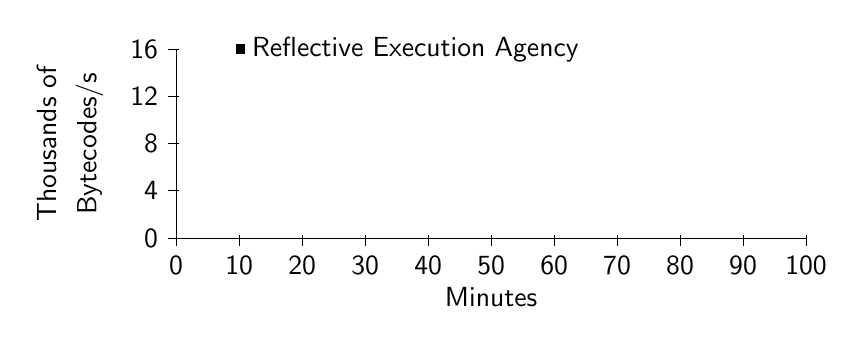
\begin{tikzpicture}[y=0.15cm, x=\experimentxscale,font=\sffamily]
 	%axis
	\draw (0,0) -- coordinate (x axis mid) (\experimentxaxismax,0);
    	\draw (0,0) -- coordinate (y axis mid) (0,16);
    	%ticks
    	\foreach \x in {0,\experimentxaxispertick,...,\experimentxaxismax}
     		\draw (\x,1pt) -- (\x,-3pt)
			node[anchor=north] {\x};
    	\foreach \y in {0,4,...,16}
     		\draw (1pt,\y) -- (-3pt,\y) 
     			node[anchor=east] {\y}; 
        
	%labels
	\node[below=0.5cm] at (x axis mid) {Minutes};
	\node[rotate=90, above=1.4cm] at (y axis mid) {Thousands of};
	\node[rotate=90, above=0.8cm] at (y axis mid) {Bytecodes/s};

	%plots
	\draw plot[mark=square*, mark options={fill=black,scale=\experimentmarkscale}]
		file {data/mind_plot-Gripper-1-reflective-execution-bytecode_count.data};
        
	%legend
	\begin{scope}[shift={(10,16)}]
	\draw (0,0) -- 
		plot[mark=square*, mark options={fill=black,scale=\experimentmarkscale}] (0.25,0) -- (0.5,0) 
		node[right]{Reflective Execution Agency};
	\end{scope}
\end{tikzpicture}

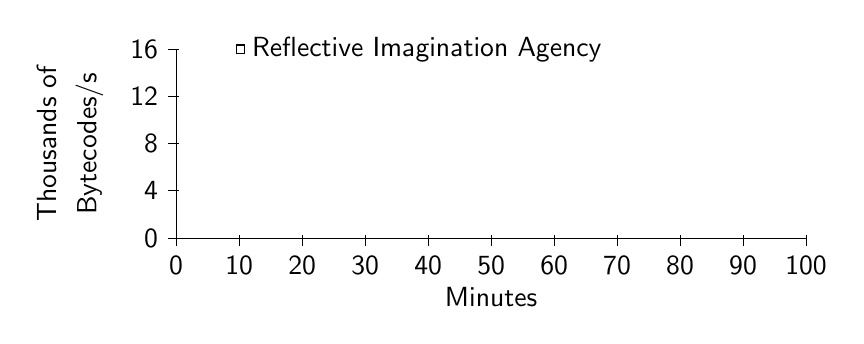
\begin{tikzpicture}[y=0.15cm, x=\experimentxscale,font=\sffamily]
 	%axis
	\draw (0,0) -- coordinate (x axis mid) (\experimentxaxismax,0);
    	\draw (0,0) -- coordinate (y axis mid) (0,16);
    	%ticks
    	\foreach \x in {0,\experimentxaxispertick,...,\experimentxaxismax}
     		\draw (\x,1pt) -- (\x,-3pt)
			node[anchor=north] {\x};
    	\foreach \y in {0,4,...,16}
     		\draw (1pt,\y) -- (-3pt,\y) 
     			node[anchor=east] {\y}; 
        
	%labels
	\node[below=0.5cm] at (x axis mid) {Minutes};
	\node[rotate=90, above=1.4cm] at (y axis mid) {Thousands of};
	\node[rotate=90, above=0.8cm] at (y axis mid) {Bytecodes/s};

	%plots
	\draw plot[mark=square*, mark options={fill=white,scale=\experimentmarkscale}]
		file {data/mind_plot-Gripper-1-reflective-imagination-bytecode_count.data};
        
	%legend
	\begin{scope}[shift={(10,16)}]
	\draw (0,0) -- 
		plot[mark=square*, mark options={fill=white,scale=\experimentmarkscale}] (0.25,0) -- (0.5,0) 
		node[right]{Reflective Imagination Agency};
	\end{scope}
\end{tikzpicture}

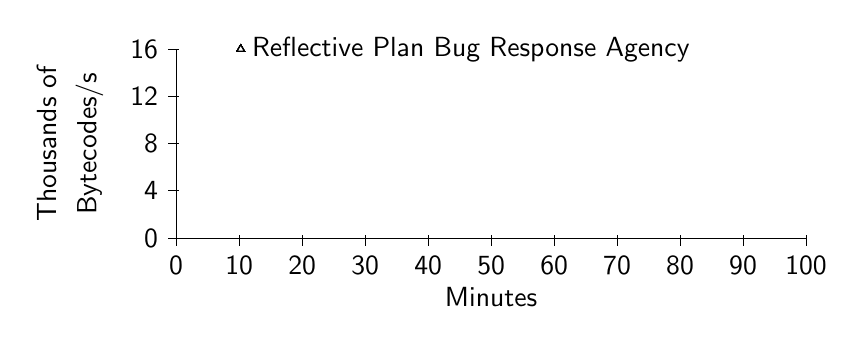
\begin{tikzpicture}[y=0.15cm, x=\experimentxscale,font=\sffamily]
 	%axis
	\draw (0,0) -- coordinate (x axis mid) (\experimentxaxismax,0);
    	\draw (0,0) -- coordinate (y axis mid) (0,16);
    	%ticks
    	\foreach \x in {0,\experimentxaxispertick,...,\experimentxaxismax}
     		\draw (\x,1pt) -- (\x,-3pt)
			node[anchor=north] {\x};
    	\foreach \y in {0,4,...,16}
     		\draw (1pt,\y) -- (-3pt,\y) 
     			node[anchor=east] {\y}; 
        
	%labels
	\node[below=0.5cm] at (x axis mid) {Minutes};
	\node[rotate=90, above=1.4cm] at (y axis mid) {Thousands of};
	\node[rotate=90, above=0.8cm] at (y axis mid) {Bytecodes/s};

	%plots
	\draw plot[mark=triangle*, mark options={fill=white,scale=\experimentmarkscale}]
		file {data/mind_plot-Gripper-1-reflective-plan_bug_response-bytecode_count.data};
        
	%legend
	\begin{scope}[shift={(10,16)}]
	\draw (0,0) -- 
		plot[mark=triangle*, mark options={fill=white,scale=\experimentmarkscale}] (0.25,0) -- (0.5,0) 
		node[right]{Reflective Plan Bug Response Agency};
	\end{scope}
\end{tikzpicture}

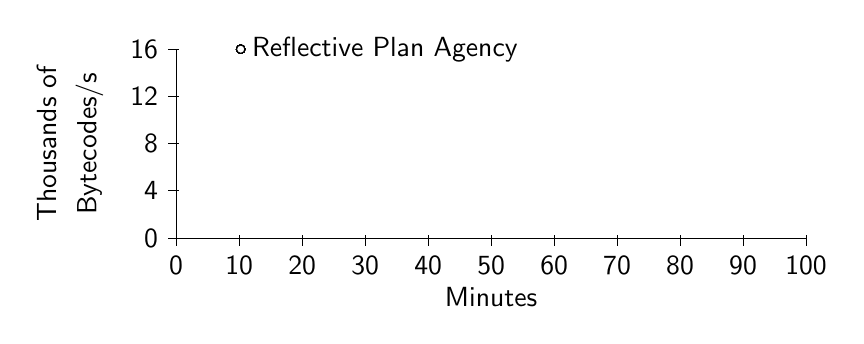
\begin{tikzpicture}[y=0.15cm, x=\experimentxscale,font=\sffamily]
 	%axis
	\draw (0,0) -- coordinate (x axis mid) (\experimentxaxismax,0);
    	\draw (0,0) -- coordinate (y axis mid) (0,16);
    	%ticks
    	\foreach \x in {0,\experimentxaxispertick,...,\experimentxaxismax}
     		\draw (\x,1pt) -- (\x,-3pt)
			node[anchor=north] {\x};
    	\foreach \y in {0,4,...,16}
     		\draw (1pt,\y) -- (-3pt,\y) 
     			node[anchor=east] {\y}; 
	%labels
	\node[below=0.5cm] at (x axis mid) {Minutes};
	\node[rotate=90, above=1.4cm] at (y axis mid) {Thousands of};
	\node[rotate=90, above=0.8cm] at (y axis mid) {Bytecodes/s};

	%plots
	\draw plot[mark=*, mark options={fill=white,scale=\experimentmarkscale}]
		file {data/mind_plot-Gripper-1-reflective-plan-bytecode_count.data};
        
	%legend
	\begin{scope}[shift={(10,16)}]
	\draw (0,0) -- 
		plot[mark=*, mark options={fill=white,scale=\experimentmarkscale}] (0.25,0) -- (0.5,0) 
		node[right]{Reflective Plan Agency};
	\end{scope}
\end{tikzpicture}

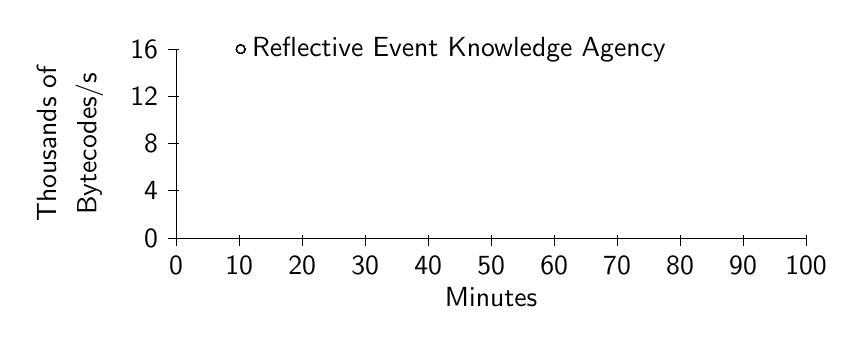
\begin{tikzpicture}[y=0.15cm, x=\experimentxscale,font=\sffamily]
 	%axis
	\draw (0,0) -- coordinate (x axis mid) (\experimentxaxismax,0);
    	\draw (0,0) -- coordinate (y axis mid) (0,16);
    	%ticks
    	\foreach \x in {0,\experimentxaxispertick,...,\experimentxaxismax}
     		\draw (\x,1pt) -- (\x,-3pt)
			node[anchor=north] {\x};
    	\foreach \y in {0,4,...,16}
     		\draw (1pt,\y) -- (-3pt,\y) 
     			node[anchor=east] {\y}; 
	%labels
	\node[below=0.5cm] at (x axis mid) {Minutes};
	\node[rotate=90, above=1.4cm] at (y axis mid) {Thousands of};
	\node[rotate=90, above=0.8cm] at (y axis mid) {Bytecodes/s};

	%plots
	\draw plot[mark=*, mark options={fill=white,scale=\experimentmarkscale}]
		file {data/mind_plot-Gripper-1-reflective-reflective_event_knowledge-bytecode_count.data};
        
	%legend
	\begin{scope}[shift={(10,16)}]
	\draw (0,0) -- 
		plot[mark=*, mark options={fill=white,scale=\experimentmarkscale}] (0.25,0) -- (0.5,0) 
		node[right]{Reflective Event Knowledge Agency};
	\end{scope}
\end{tikzpicture}
\caption[Rate of bytecode execution in each agency of the reflective
  layer of the AI during a demonstration.]{Rate of bytecode execution
  in each agency of the reflective layer of the AI during a
  demonstration of mind initialization, plan execution, failure,
  physical learning, and reflective learning.}
\label{figure:mind_plot_data}
\end{figure}


% reflective agency memory allocation rate plots
\begin{figure}
\raggedleft
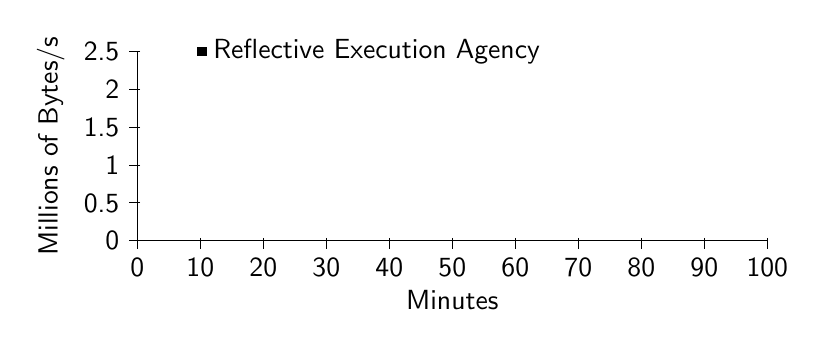
\begin{tikzpicture}[y=0.96cm, x=\experimentxscale,font=\sffamily]
 	%axis
	\draw (0,0) -- coordinate (x axis mid) (\experimentxaxismax,0);
    	\draw (0,0) -- coordinate (y axis mid) (0,2.5);
    	%ticks
    	\foreach \x in {0,\experimentxaxispertick,...,\experimentxaxismax}
     		\draw (\x,1pt) -- (\x,-3pt)
			node[anchor=north] {\x};
    	\foreach \y in {0,0.5,...,2.5}
     		\draw (1pt,\y) -- (-3pt,\y) 
     			node[anchor=east] {\y}; 
        
	%labels
	\node[below=0.5cm] at (x axis mid) {Minutes};
	\node[rotate=90, above=0.8cm] at (y axis mid) {Millions of Bytes/s};

	%plots
	\draw plot[mark=square*, mark options={fill=black,scale=\experimentmarkscale}]
		file {data/mind_plot-Gripper-1-reflective-execution-bytes_allocated_count.data};
        
	%legend
	\begin{scope}[shift={(10,2.5)}]
	\draw (0,0) -- 
		plot[mark=square*, mark options={fill=black,scale=\experimentmarkscale}] (0.25,0) -- (0.5,0) 
		node[right]{Reflective Execution Agency};
	\end{scope}
\end{tikzpicture}

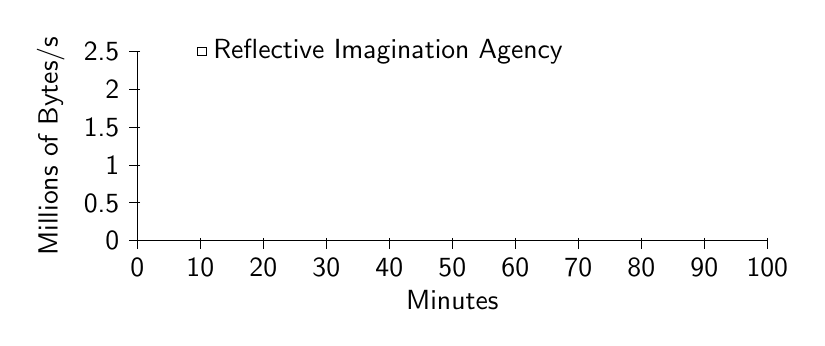
\begin{tikzpicture}[y=0.96cm, x=\experimentxscale,font=\sffamily]
 	%axis
	\draw (0,0) -- coordinate (x axis mid) (\experimentxaxismax,0);
    	\draw (0,0) -- coordinate (y axis mid) (0,2.5);
    	%ticks
    	\foreach \x in {0,\experimentxaxispertick,...,\experimentxaxismax}
     		\draw (\x,1pt) -- (\x,-3pt)
			node[anchor=north] {\x};
    	\foreach \y in {0,0.5,...,2.5}
     		\draw (1pt,\y) -- (-3pt,\y) 
     			node[anchor=east] {\y}; 
        
	%labels
	\node[below=0.5cm] at (x axis mid) {Minutes};
	\node[rotate=90, above=0.8cm] at (y axis mid) {Millions of Bytes/s};
        
	%plots
	\draw plot[mark=square*, mark options={fill=white,scale=\experimentmarkscale}]
		file {data/mind_plot-Gripper-1-reflective-imagination-bytes_allocated_count.data};
        
	%legend
	\begin{scope}[shift={(10,2.5)}]
	\draw (0,0) -- 
		plot[mark=square*, mark options={fill=white,scale=\experimentmarkscale}] (0.25,0) -- (0.5,0) 
		node[right]{Reflective Imagination Agency};
	\end{scope}
\end{tikzpicture}

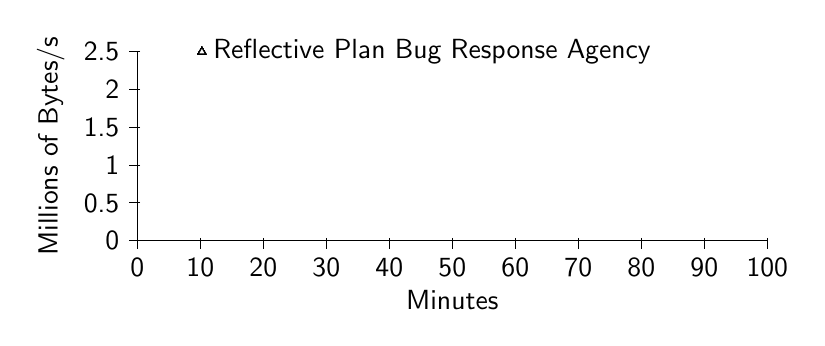
\begin{tikzpicture}[y=0.96cm, x=\experimentxscale,font=\sffamily]
 	%axis
	\draw (0,0) -- coordinate (x axis mid) (\experimentxaxismax,0);
    	\draw (0,0) -- coordinate (y axis mid) (0,2.5);
    	%ticks
    	\foreach \x in {0,\experimentxaxispertick,...,\experimentxaxismax}
     		\draw (\x,1pt) -- (\x,-3pt)
			node[anchor=north] {\x};
    	\foreach \y in {0,0.5,...,2.5}
     		\draw (1pt,\y) -- (-3pt,\y) 
     			node[anchor=east] {\y}; 
        
	%labels
	\node[below=0.5cm] at (x axis mid) {Minutes};
	\node[rotate=90, above=0.8cm] at (y axis mid) {Millions of Bytes/s};

	%plots
	\draw plot[mark=triangle*, mark options={fill=white,scale=\experimentmarkscale}]
		file {data/mind_plot-Gripper-1-reflective-plan_bug_response-bytes_allocated_count.data};
        
	%legend
	\begin{scope}[shift={(10,2.5)}]
	\draw (0,0) -- 
		plot[mark=triangle*, mark options={fill=white,scale=\experimentmarkscale}] (0.25,0) -- (0.5,0) 
		node[right]{Reflective Plan Bug Response Agency};
	\end{scope}
\end{tikzpicture}

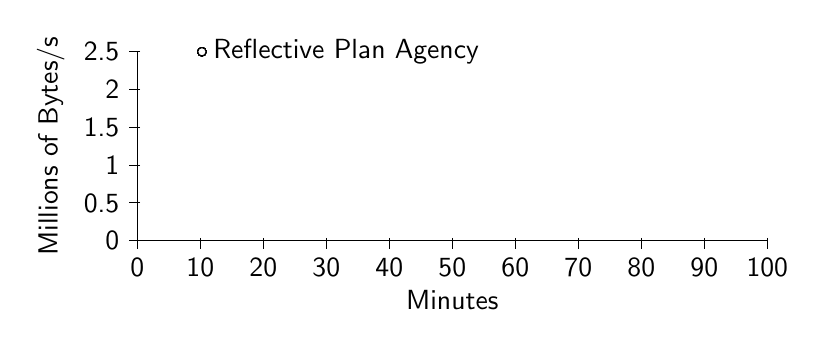
\begin{tikzpicture}[y=0.96cm, x=\experimentxscale,font=\sffamily]
 	%axis
	\draw (0,0) -- coordinate (x axis mid) (\experimentxaxismax,0);
    	\draw (0,0) -- coordinate (y axis mid) (0,2.5);
    	%ticks
    	\foreach \x in {0,\experimentxaxispertick,...,\experimentxaxismax}
     		\draw (\x,1pt) -- (\x,-3pt)
			node[anchor=north] {\x};
    	\foreach \y in {0,0.5,...,2.5}
     		\draw (1pt,\y) -- (-3pt,\y) 
     			node[anchor=east] {\y}; 
        
	%labels
	\node[below=0.5cm] at (x axis mid) {Minutes};
	\node[rotate=90, above=0.8cm] at (y axis mid) {Millions of Bytes/s};

	%plots
	\draw plot[mark=*, mark options={fill=white,scale=\experimentmarkscale}]
		file {data/mind_plot-Gripper-1-reflective-plan-bytes_allocated_count.data};
        
	%legend
	\begin{scope}[shift={(10,2.5)}]
	\draw (0,0) -- 
		plot[mark=*, mark options={fill=white,scale=\experimentmarkscale}] (0.25,0) -- (0.5,0) 
		node[right]{Reflective Plan Agency};
	\end{scope}
\end{tikzpicture}

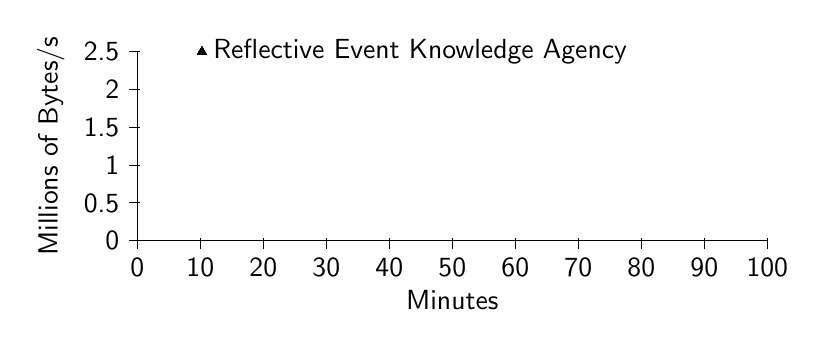
\begin{tikzpicture}[y=0.96cm, x=\experimentxscale,font=\sffamily]
 	%axis
	\draw (0,0) -- coordinate (x axis mid) (\experimentxaxismax,0);
    	\draw (0,0) -- coordinate (y axis mid) (0,2.5);
    	%ticks
    	\foreach \x in {0,\experimentxaxispertick,...,\experimentxaxismax}
     		\draw (\x,1pt) -- (\x,-3pt)
			node[anchor=north] {\x};
    	\foreach \y in {0,0.5,...,2.5}
     		\draw (1pt,\y) -- (-3pt,\y) 
     			node[anchor=east] {\y}; 
        
	%labels
	\node[below=0.5cm] at (x axis mid) {Minutes};
	\node[rotate=90, above=0.8cm] at (y axis mid) {Millions of Bytes/s};

	%plots
	\draw plot[mark=triangle*, mark options={fill=black,scale=\experimentmarkscale}]
		file {data/mind_plot-Gripper-1-reflective-reflective_event_knowledge-bytes_allocated_count.data};
        
	%legend
	\begin{scope}[shift={(10,2.5)}]
	\draw (0,0) -- 
		plot[mark=triangle*, mark options={fill=black,scale=\experimentmarkscale}] (0.25,0) -- (0.5,0) 
		node[right]{Reflective Event Knowledge Agency};
	\end{scope}
\end{tikzpicture}
\caption[Rate of memory allocation in each agency of the reflective
  layer of the AI during a demonstration.]{Rate of memory allocation
  in each agency of the reflective layer of the AI during a
  demonstration of mind initialization, plan execution, failure,
  physical learning, and reflective learning.}
\label{figure:mind_plot_data}
\end{figure}





\section{The Implementation}

The computational implementation described in
{\mbox{\autoref{part:the_implementation}}} serves the following
purposes:
\begin{enumerate}
\item To describe $n$ layers of procedurally reflective heuristic
  learning that do not affect the ``big O'' time complexity of the
  algorithm under focus.
\item To describe $n$ layers of planning machines that operate by
  executing a number of simple constant time, $O(1)$, planning
  activities that are combined in order to perform all search-like
  operations within the model, avoiding any primitives that would
  imply declarative or logical searches ``behind the scenes'', so that
  all search-like activities may be reflectively optimized.
\item To describe $n$ layers of efficient causal hypothesis learning
  and knowledge maintenance from the failure of counterfactual
  decisions back to bases in factual perceptual memories.  In this
  way, planning heuristics are defined to be hypotheses of planning
  machine operations by the reflective thinking layers of second-order
  and above.
\end{enumerate}
There are two key features that must be evaluated in the
implementation: (1) reflecting over a basic planning algorithm does
not slow down the basic planning algorithm, and (2) reflective
learning improves the efficiency of the basic planning algorithm.  I
will discuss how and when these two points are true in general.  Also,
there is a question as to increased space complexity required by each
layer of reflection.  Evaluations of these issues will be covered in
the following sections.

\section{No Theoretical Slowdown of Original Algorithm}

In order to assume that there is no theoretical slowdown of the
original planning algorithm when reflective heuristic learning is
applied, it must be assumed that the reflective implementation is an
ideal concurrent shared memory architecture.  In practice, the
underlying Funk virtual operating system slows down when more
concurrent and parallel fibers are executing.  This is beside the
theoretical point of this thesis, but the following table shows a
real-time test of the actual slowdown experienced by the Funk
operating system as different numbers of parallel fiber tasks are
executed to perform a simple numerical processing task.  The test was
done on a dual Pentium processor computer, each with ``core duo''
technology with each core implementing ``hyper-threading'', which ends
up appearing as eight processors to the Linux operating system
underlying the Funk virtual operating system:

\vspace{5mm}
\begin{tabular}{ll}
Tasks & Real-Time (s) \\
1 & 29\\
2 & 36\\
3 & 46\\
4 & 44\\
5 & 68\\
6 & 67\\
7 & 73\\
8 & 110\\
\end{tabular}
\vspace{5mm}

If a non-reflective learning algorithm is running on this hardware
implementation of a concurrent shared memory architecture and uses one
fiber and each reflective learning algorithm uses an additional fiber,
the Funk virtual operating system underlying SALS will experience
slowdown similar to that shown in this table.

\section{All Activities are Performed in Constant Time}

In order for all activities in my model to be reflectively optimized
by the $n$ layers of procedural reflective learning and planning, all
activities must be composed of primitive activities that are known to
complete in constant time, $O(1)$.  I have clearly described a
planning machine that operates based on constant time operations,
similar to a virtual machine.

In order to maintain this invariant in every aspect of the
implementation, I have needed to make some limiting assumptions in
order to avoid the general NP-complete problem of subgraph isomorphism
as a means of implementing symbolic perception.  If symbolic
perception is implemented as a subgraph isomorphism, then the
reflective optimization benefits of my model of reflective thinking no
longer apply.  In order to avoid this dangerous problem in my
implementation, I have made two temporary proof-of-concept simplifying
assumptions: (1) restricting learned symbolic perceptions to subgraphs
of 4 nodes and 4 edges or less of a constant upper-bound in
complexity, and (2) by hand-coding a small number of procedural
critics in the second-order reflective thinking layer that observe
specific properties of plans, such as similarly restricted subgraph
combinations of expected transframe additions and removals of plans in
different planning machine registers.

The general solution to the problem of symbolic perception in my model
is the planning-to-perceive problem as described by
\cite{pryorcollins:1995}.  In this way, the first-order planning
machine is responsible for creating plans that can be compiled into
perceptual resources that are composed of constant time, $O(1)$, steps
that respond to the perceptual event stream originating from the
layers below.  These plans must be composed of actions that traverse
and compare node and edge labels of the event stream as well as the
reflectively reconstructed representation of the layers below in order
to implement different planned ways to recognize the same symbol
depending on the order of the events in the stream.

It is imperative to not confuse the symbolic perception problem in my
model with the general NP-complete subgraph isomorphism problem.  In
this way, every aspect of my model, including symbolic perception,
recognizing isomorphic subgraphs in the layers below, becomes a
problem that can be optimized through procedural reflection, depending
on the order of reflective events.

\section{Efficiency Gains of Heuristic Learning}

\cite{mitchell:1997} defines the \emph{inductive learning hypothesis}
as follows:
\begin{definition}\emph{
\emph{The inductive learning hypothesis.} Any hypothesis found to
approximate the target function well over a sufficiently large set of
training examples will also approximate the target function well over
other unobserved examples.  }\end{definition} As the first-order
reflective learning algorithm learns hypotheses that generalize the
effects of actions from symbolic perceptions, the inductive learning
hypothesis is assumed of the target $\text{reflective}^0$ or physical
layer under the reflective focus.  In order to see efficiency gains in
the second-order reflective learning layer, I define here the
\emph{reflective inductive learning hypothesis}:
\begin{definition}\emph{
\emph{The reflective inductive learning hypothesis.} Any heuristic
found to approximate the target planning failure well over a
sufficiently large set of plan execution examples will also
approximate the target execution failure well over other unobserved
plan executions.}\end{definition} As long as the reflective inductive
learning hypothesis holds for a given planning domain, arbitrarily
greater planning efficiencies can be expected for each reflective
layer where this hypothesis holds true.

\section{Comparing Temporal and Reflective Learning}

A reflective learning algorithm implies arbitrarily better learning
algorithms, including one-shot learning algorithms.  In many domains,
the opportunity to learn is rare.  When the cost of failure is high,
it is important to learn as much as possible from each failure.

I will refer to machine learning algorithms that learn by assigning
credit for failures to the temporally previous action as
\emph{temporal learning} algorithms.  Contemporary temporal learning
algorithms are relatively advanced, some even having relational
object-oriented models of actions and the world.  Temporal learning
algorithms learn by assigning credit for a failure to the previous
time step or the previous action.  A reinforcement learning algorithm
that learns in this immediately temporal sense is called the
\emph{temporal difference learning} algorithm as described by
\cite*{kaelbling:1996}.  In temporal learning, the previous physical
action is considered in the context of the previous physical state of
the world.  Preconditions and postconditions for the action are
updated.  In other words, the categories of the world are updated for
this action, given the unexpected reward or punishment, a failure in
expectations.  In the temporal difference learning algorithm, there is
a focus on the previous physical action and physical state combination
in order to assign credit for failures.  Temporal learning algorithms
assign credit back, sequentially in time, from action to action.

Reflective learning algorithms can be thought of as having a temporal
learning algorithm within each necessarily distinct layer of
knowledge.  Reflective learning can take advantage of concurrent
processors for each separate layer of activity without slowing down
the primary learning algorithm under focus.  Let $n$ be the number of
reflective layers in a learning algorithm with each layer on a
concurrent processor.  If there is a memory of actions and the state
of the world for the previous time step, a temporal learning algorithm
spends $O(1)$ time relearning the effects of the temporally previous
action.  This process can be repeated for probabilistic algorithms,
resulting in a statistical spreading of credit through the uncertainty
of a number of previous actions.  The reflective algorithm also spends
$O(1)$ time but relearns the effects of $n$ actions, where $n$ is
limited by memory and processors.
{\mbox{\autoref{figure:learning_complexities}}} shows a comparison of
the time and space complexities of temporal and reflective learning
algorithms as well as the number of learning opportunities afforded by
one failure.
\begin{figure}
\center
\begin{tabular}{p{2cm}|p{2cm}|p{2cm}|p{3cm}}
Learning Algorithm & Time   & Space  & One-shot Learning Opportunities \\ \hline
Temporal           & $O(1)$ & $O(1)$ & $1$ \\
Reflective         & $O(1)$ & $O(n)$ & $n$ \\
\end{tabular}
\caption{Temporal and reflective learning complexities with one-shot learning opportunities.}
\label{figure:learning_complexities}
\end{figure}



\begin{figure}
\center
\begin{tikzpicture}[y=.2cm, x=.7cm,font=\sffamily]
 	%axis
	\draw (0,0) -- coordinate (x axis mid) (10,0);
    	\draw (0,0) -- coordinate (y axis mid) (0,30);
    	%ticks
    	\foreach \x in {0,...,10}
     		\draw (\x,1pt) -- (\x,-3pt)
			node[anchor=north] {\x};
    	\foreach \y in {0,5,...,30}
     		\draw (1pt,\y) -- (-3pt,\y) 
     			node[anchor=east] {\y}; 
	%labels      
	\node[below=0.8cm] at (x axis mid) {MOPS};
	\node[rotate=90, above=0.8cm] at (y axis mid) {Power [mW]};

	%plots
	\draw plot[mark=*, mark options={fill=white}] 
		file {div_soft.data};
	\draw plot[mark=triangle*, mark options={fill=white} ] 
		file {div_ciu.data};
	\draw plot[mark=square*, mark options={fill=white}]
		file {div_ciu_oscar.data};
	\draw plot[mark=square*]
		file {div_ciu_oscar_extrapolated.data};  
    
	%legend
	\begin{scope}[shift={(4,4)}] 
	\draw (0,0) -- 
		plot[mark=*, mark options={fill=white}] (0.25,0) -- (0.5,0) 
		node[right]{soft};
	\draw[yshift=\baselineskip] (0,0) -- 
		plot[mark=triangle*, mark options={fill=white}] (0.25,0) -- (0.5,0)
		node[right]{ciu};
	\draw[yshift=2\baselineskip] (0,0) -- 
		plot[mark=square*, mark options={fill=white}] (0.25,0) -- (0.5,0)
		node[right]{ciu + oscar};
	\draw[yshift=3\baselineskip] (0,0) -- 
		plot[mark=square*, mark options={fill=black}] (0.25,0) -- (0.5,0)
		node[right]{ciu + oscar extrapolated};
	\end{scope}
\end{tikzpicture}
\caption{Sample tikz plot.}
\label{figure:sample_tikz}
\end{figure}

\section{Space Complexity}

\section{Conclusion}



